\chapter{АНАЛИЗ И УВЕЛИЧЕНИЕ ПРОИЗВОДИТЕЛЬНОСТИ БЕСПРОВОДНЫХ ЦЕНТРАЛИЗОВАННЫХ СЕТЕЙ ДЛЯ ПЕРЕДАЧИ НЕАДАПТИВНЫХ ВИДЕОПОТОКОВ}
\label{chap3}

\section{Вводные замечания}
\label{chap3:Intro}
В настоящее время в беспроводных сетях, несмотря на бурное развитие технологий адаптивной передачи видеоконтента, достаточно распространена передача видео с использованием неадаптивных видеоплееров. Наиболее ярким примером является социальная сеть Facebook, весь видеоконтент которой представлен в двух репрезентациях: стандартном и высоком разрешениях, в англоязычной терминологии Standard Definition и High Definition соотвественно. Пользователь при просмотре видео может выбрать один из двух представленных выше вариантов качества видеопотока и оно не будет изменяться во времени. Подобная модель поведения полностью соответствует описанию неадаптивного видеоплеера, представленного в подразделе~\ref{chap1:VideoPlayers}.

В настоящем разделе производится аналитическое исследование производительности беспроводных централизованных систем передачи информации с доминированием передачи видеоданных по протоколу прикладного уровня HTTP. В начале раздела предлагается критерий качества обслуживания для неадаптивных видеопотоков. Далее вводится дополнительные допущения, специфичные для неадаптивных видеопоследовательностей. Затем формулируется оптимизационная задача и предлагается нижняя граница для введенного критерия качества обслуживания. В завершении предлагается численный пример, демонстрирующий производительность стандартных алгоритмов планирования распределения ресурсов беспроводного канала по сравнению с полученной нижней границей.

Основные результаты данного раздела опубликованы в работах~\cite{past_tur,Suai2017}.

\section{Критерий качества восприятия неадаптивного видеопотока}
\label{chap3:NonAdaptiveQoe}
Обобщая информацию, представленную ранее в настоящей работе, можно выделить три основных фактора, влияющих на восприятие видеопоследовательности:
\begin{itemize}
	\item Репрезентация (рекомендуемое разрешение экрана и частота кадров видео), определяемая битовой скоростью потока (подраздел~\ref{chap1:VideoMOS}).
	\item Прерывание воспроизведения, вызванное буферизацией видеопотока, включающее начальную буферизацию видео (подраздел~\ref{chap1:VideoMOS});
	\item Гладкость воспроизведения видеопоследовательности~--~частота изменения битовой скорости во времени (подраздел~\ref{chap2:VideoTrafficModel}).
\end{itemize}
Рассмотрим каждый из перечисленных выше факторов с точки зрения неадаптивных видеопоследовательностей.

При работе неадаптивного видеоплеера решение о выборе репрезентации видеоряда принимает пользователь некоторым образом, отвечающим индивидуальным требованиям к качеству просматриваемого видео и не изменяет его во времени. Из неизменности репрезентации видео во времени, следует что гладкость воспроизведения, которая характеризует частоту изменения репрезентации во времени, не влияет на качество восприятия видеоряда.

Таким образом, на удовлетворенность пользователя от просмотра неадаптивных видеопоследовательностей влияют прерывания воспроизведения, вызванные опустошением буфера и начальной буферизацией на пользовательском устройстве.

Очевидно, что если в соте находится большое число абонентов, то могут проявится эффекты деградации воспроизведения видео у пользователей, ввиду конечности количества частотно-временных ресурсов беспроводного канала и ограниченности снизу минимальной битовой скорости репрезентации видео. Например, если некоторому пользователю базовая станция обеспечивает скорость загрузки информации равную $0.25$ Мбит/с, а битовая скорость минимальной репрезентации равняется $0.5$ Мбит/с, то у данного пользователя при просмотре видео с высокой вероятностью будет длительная начальная буферизация и неизбежно возникнут прерывания воспроизведения видео. Основываясь на данном факте, введем определение перегрузки:
\begin{definition}
\label{def:Congestion}
    \emph{Перегрузка}~--~состояние системы передачи информации, характеризующее недостаток ресурсов для обеспечения достаточного уровня удовлетворенности всех активных пользователей.
\end{definition}

Как было представлено в подразделе~\ref{chap2:GeneralOverview}, все время $T$ нахождения пользователя в системе разделено на три фазы: буферизация $\left( b_i^T \right)$, просмотр $\left( w_i^T \right)$ и паузы между просмотрами видео $\left( p_i^T \right)$. В настоящем разделе предлагается оценивать качество восприятия видеопотока для пользователя как нормированное отношение длительностей буферизации и просмотра за время $T$:
\begin{definition}
\label{def:gMetric}
    \emph{Нормированное отношение длительностей буферизации и просмотра} для пользователя $i$~--~это отношение общей длительности буферизации к длительности нахождения пользователя в системе, исключая паузы между просмотрами видео:
    \emph{
    \begin{equation}
    	\label{eq:gMetric}
		g_i = \lim\limits_{T\rightarrow\infty} \frac{b_i^T}{w_i^T + b_i^T}.
	\end{equation}
	}
\end{definition}

Критерий восприятия (\ref{eq:gMetric}) описывает процентное соотношение общих длительностей буферизации и просмотра для пользователя $i$. На основе данного критерия возможно оценить удовлетворенность пользователя следующим образом:
$$g_i=
\begin{cases}
0, & \text{пользователь $i$ удовлетворен просмотром}\\
\varepsilon \in (0,1) & \text{пользователь $i$ наблюдает негативные эффекты при просмотре}\\
1, & \text{пользователь $i$ полностью неудовлетворен просмотром}\\
\end{cases}.
$$
Если пользователь не ожидал в течение времени нахождения в системе $\left(b_i^T = 0\right)$, тогда значение $g_i = 0$.
Если пользователь за время $T$ не просмотрел ни одной секунды видео $\left(w_i^T = 0\right)$, то значение $g_i$ будет равно $1$. Изначально критерий (определение \ref{def:gMetric}) был предложен в работе \cite{QoE_enhancement}, в англоязычной литературе данный критерий известен под названием \textit{<<rebuffering percentage>>}. Термин \textit{<<rebuffering>>} в англоязычной литературе используется для обозначения времени ожидания воспроизведения в течении просмотра видео при передаче с использованием протокола HTTP.

В качестве критерия качества работы системы в целом предлагается использовать среднее значение отношения длительностей буферизации и просмотра по всем пользователям, присутствующих в системе: $\bar{g}\left(A\right)$, где $A$~--~является некоторым алгоритмом планирования на базовой станции. Важно отметить, что значение критерия качества обслуживания имеет прямую зависимость от испоьзуемого алгоритма планирования распределения ресурсов беспроводного канала $A$.

После определения критерия качества обслуживания в дальнейшем будет произведена постановка оптимизационной задачи.

\section{Постановка оптимизационной задачи}
\label{chap3:NonAdaptiveOptimizationProblem}

В настоящем подразделе будет продолжено рассмотрение критерия качества обслуживания для неадаптивных видеопотоков, введенного в подразделе~\ref{chap3:NonAdaptiveQoe}. На основе проведенного рассмотрения будет предложена постановка оптимизационной задачи, решение которой характеризует максимальную возможную производительность алгоритма планирования при передаче неадаптивных видеопотоков.

Рассмотрим критерий качества для неадаптивного видео: нормированного отношения длительностей буферизации и просмотра $g_i$ (определение \ref{def:gMetric}). По определению, удовлетворенность пользователя имеет обратную корреляцию с данным критерием: чем меньше значение $g_i$, тем выше удовлетворенность пользователя $i$. Для каждого конкретного алгоритма планирования $A$, принадлежащему множеству $\mathcal{A}$, производительность возможно оценить следующим образом:
%Как следствие, основной целью увеличения производительности системы является поиск минимального значения $\bar{g}$ по всем возможным алгоритмам планирования $\mathcal{A}$, удовлетворяющих введенным допущениям:
$$\bar{g}\left(A\right) = \frac{1}{N}\left(\sum\limits_{i=1}^{N} {g_i\left(A\right)}\right).$$

Однако, множество возможных алгоритмов планирования, удовлетворяющих допущениям, является бесконечным и несчетным, поэтому вместо поиска минимального значения в данном разделе будет найдена нижняя граница (инфинум) по всем возможным алгоритмам $\mathcal{A}$:

\begin{equation}
	\label{eq:gMetricGoal}
	G = \inf\limits_{A \in \mathcal{A}} \bar{g}\left(A\right).
\end{equation}

Ранее в подразделе~\ref{chap2:GeneralOverview} было введено определение для $q_i$: отношения длительностей буферизации и просмотра для пользователя $i$ (определение~\ref{def:BWTR}). Покажем, каким образом взаимосвязаны значения $g_i$ и $q_i$. По определению данных величин, если продолжительность буферизации $\left(b_i^T\right)$ равнялась нулю, то $q_i=g_i=0$. Пусть значение $b_i^T$ отлично от нуля, тогда значения $q_i$ и $g_i$ взаимосвязаны следующим образом:
$$q_i = \frac{g_i}{1-g_i}.$$

На основе представленной выше взаимосвязи значений критериев качества обслуживания выражение (\ref{eq:GeneralConstrain}), полученное в результате доказательства Утверждения~\ref{lem:GeneralConstrain} (подраздел \ref{chap2:InterrelationVideoParams}) примет следующий вид:
\begin{equation}
	\label{eq:GeneralConstrainToG}
	\sum\limits_{i=1}^{N} {\left(1-\nu^R_i\nu^C_i\right)E[R_i]E[C_i^{-1}]\frac{1-g_i}{g_i + \gamma_i (1-g_i)}} \leq 1.
\end{equation}

При просмотре неадаптивных видеопоследовательностей пользователь $i$ в начальный момент времени выбирает репрезентацию с битовой скоростью $R_i$ и не изменят ее в течении всего времени работы. Данный факт приводит к изменению допущения \textit{Модели видеоплеера} номер $1$ , представленному в подразделе \ref{chap2:Assumptions}, следующим образом:

$1.$   Значение битовой скорости видеопотока для каждого конкретного абонента неизменно во времени: $R_{i,1} = R_{i,2} = \ldots = R_i, i=\overline{1,N}$.

Следствием из данного допущения является равенство коэффициента вариации $\nu^R_i, i=\overline{1,N}$ нулю, а математическое ожидания битовой скорости $E[R_i]$ равно $R_i$ для каждого пользователя $i$. Таким образом, неравенство (\ref{eq:GeneralConstrainToG}) принимает следующий вид:
$$\sum\limits_{i=1}^{N} {R_i E[C_i^{-1}]\frac{1-g_i}{g_i + \gamma_i (1-g_i)}} \leq 1.$$

Для уменьшения объема последующих математических преобразований введем обозначение $K_i = R_i E[C_i^{-1}]$. Важно отметить, что значение $K_i$ не является переменной, так как его компоненты задаются независимыми от оптимизации факторами: пожеланиями пользователя ($R_i$) и условиями беспроводного канала ($E[C_i^{-1}]$).

В дополнении к системе допущений \textit{Модели поведения пользователя при просмотре видео}, введенному в подразделе \ref{chap2:Assumptions}, в рамках настоящего раздела вводится дополнительное допущение:

$2.$   Коэффициент разреженности видеопотока $\gamma_i$ (определение \ref{def:VideoSparseness}) для всех пользователей имеет равное значение: $\gamma_i = \gamma, i=\overline{1,N}$.

Настоящее допущение обусловлено зависимостью в реальной системе между длительностью видеоролика и паузы после его просмотра: после просмотра длительного ролика пользователь <<осмысливает>> его более длительный промежуток времени, чем при просмотре короткого ролика. Это приводит приблизительному равенству коэффициентов разреженности потока у всех пользователей.

Обобщая сказанное выше, в настоящем разделе предлагается оптимизационная задача следующего вида:
\begin{equation}
\begin{array}{l}
\text{ \textbf{Минимизировать:} } G = \sum\limits_{i=1}^{N} {g_i} \\
\text{ \textbf{При условии:} }\\
\begin{cases}
\sum\limits_{i=1}^{N} {\frac{K_i (1-g_i)}{g_i + \gamma (1-g_i)}} \leq 1 \\
g_i \in [0,1], i=\overline{1,N}
\end{cases}
\end{array}.
\label{eq:optim_problem_g}
\end{equation}

Оптимизационная задача (\ref{eq:optim_problem_g}) является задачей нелинейного программирования, ввиду нелинейности первого ограничения. Дальнейшая часть данного раздела посвящена поиску оптимального решения задачи (\ref{eq:optim_problem_g}), значение которого задает нижнюю границу по всем возможным алгоритмам планирования, удовлетворяющих допущениям введенных в подразделе ~\ref{chap2:Assumptions}.

\section{Решение обобщенной непрерывной задачи о рюкзаке}
\label{chap3:GeneralizedFKSP}

Отыскание решения оптимизационной задачи (\ref{eq:optim_problem_g}) является сложной задачей, и для ее решения необходимо проделать несколько шагов. Изначально будет рассмотрено обобщение известной непрерывной задачи о рюкзаке и найдено его решение. Далее будет показано, каким образом найденное решение может быть использовано при решении оптимизационной задачи (\ref{eq:optim_problem_g}). В данном подразделе рассматривается непрерывная задача о рюкзаке, ее обобщение и находится решение обобщенной задачи.

Представленное ниже решение опубликовано в работе \cite{Suai2017}.

Непрерывная задача о рюкзаке в англоязычной литературе известна под термином \textit{<<fractional knapsack problem>>}, и подробно описана в \cite{Cormen:2009:IAT:1614191}. Задача формулируется следующим образом. Имеется набор из $N$ предметов, каждый предмет $i$ характеризуется двумя величинами: стоимостью $(c_i)$ и весом ($w_i$). Также имеется рюкзак неограниченного объема, характеризующийся весом предметов, помещенных в него. Считается, что человек, который будет нести этот рюкзак, не может поднять вес превышающий $W$. Все предметы считаются делимыми на бесконечное число частей, что позволяет выбрать долю каждого предмета $x_i$, которую он положит в рюкзак. В качестве задачи, предлагается найти такой вектор $(x_1, x_2, \ldots, x_N)$, что вес взятых долей предметов не превышает $W$ и при этом стоимость взятых предметов максимальна. Математическое представление непрерывной задачи о рюкзаке представлено системой (\ref{eq:fksp}).

\begin{equation}
\begin{array}{l}
\text{ \textbf{Максимизировать:} } \sum\limits_{i=1}^{N} {c_i x_i} \\
\text{ \textbf{При условии:} }\\
\begin{cases}
\sum\limits_{i=1}^{N} {w_i x_i} \leq W \\
x_i \in \left[0,1\right], & i=\overline{1,N}
\end{cases}
\end{array}.
\label{eq:fksp}
\end{equation}
Таким образом, непрерывная задача о рюкзаке относится к классу непрерывных задач линейного программирования от нескольких переменных.

Важным отличием непрерывной задачи о рюкзаке (\ref{eq:fksp}) от классической задачи о рюкзаке (\textit{<<0-1 knapsack problem>>}) заключается в возможности деления предметов, когда в классической задаче предметы считаются неделимыми (величина $x_i$ может принимать только два значения: $0$ и $1$). Известно, что задача о рюкзаке не имеет замкнутого решения и может быть решена методами динамического программирования. Однако, для непрерывной задачи о рюкзаке оптимальное решение может быть получено <<жадным алгоритмом>> (алгоритм \ref{alg:algorithm_lemma}) \cite{Cormen:2009:IAT:1614191}.

\begin{algorithm}
  \caption{: Решение непрерывной задачи о рюкзаке}
	\label{alg:algorithm_lemma}
  \begin{algorithmic}[1]
	 \item Сортировка предметов по возрастанию отношений $\frac{w_i}{c_i}$, и их нумерация, в соответствие с сортировкой;
	 \item Нахождение предмета с индексом $j:\begin{cases}
		\sum\limits_{i=1}^{j-1} {w_i} \leq W \\
		\sum\limits_{i=1}^{j} {w_i} > W
		\end{cases}$
		\newline
		Если $j\in\varnothing$, то $j=N+1$;
	\item Нахождение оптимальных значений $x_i$: \newline
	$x_i=\begin{cases}
		1, & i < j \\
		\frac{1}{w_j}\left(W - \sum\limits_{i=1}^{j-1} {w_i}\right), & i=j \\
		0, & i > j
		\end{cases}$.
  \end{algorithmic}
\end{algorithm}

Настоящий подраздел организован следующим образом. Первым шагом, будет представлено обобщение непрерывной задачи о рюкзаке. Вторым шагом будет показано каким образом алгоритм \ref{alg:algorithm_lemma} может быть применен для решения обобщенной непрерывной задачи о рюкзаке. В завершении подраздела будет представлено сравнение сложности полученного решения со стандартными методами решения задач выпуклого программирования от нескольких переменных.

Обобщение непрерывной задачи о рюкзаке:
\begin{equation}
\begin{array}{l}
\text{ \textbf{Максимизировать:} } \sum\limits_{i=1}^{N} {f(x_i)} \\
\text{ \textbf{При условии:} }\\
\begin{cases}
\sum\limits_{i=1}^{N} {w_i x_i} \leq W \\
x_i \in \left[0,1\right], & i=\overline{1,N}
\end{cases}
\end{array},
\label{eq:fksp_general}
\end{equation}
где $f(x_i)$~--~непрерывная, дважды дифференцируемая, строго монотонно возрастающая, выпуклая вниз функция, ограниченная сверху и снизу в области определения $x_i$.

Оптимизационная задача (\ref{eq:fksp_general}) относится к классу выпуклого программирования от нескольких переменных с ограничениями типа неравенства. Важно отметить факт, что задачи выпуклого программирования являются подклассом задач нелинейного программирования.

Решение оптимизационной задачи (\ref{eq:fksp_general}) описывается в утверждении \ref{lem:fksp_general_lemma}.

\begin{lemma}
\label{lem:fksp_general_lemma}
Если в алгоритме \ref{alg:algorithm_lemma} принять $\forall i: c_i = 1$, то вектор $X = (x_1, x_2, \ldots, x_N)$, полученный в результате выполнения алгоритма \ref{alg:algorithm_lemma}, является решением задачи нелинейного программирования (\ref{eq:fksp_general}).
\end{lemma}

\begin{proof}

В основе предложенного далее доказательства был использован метод от противного. Предположим, что существует оптимальное решение $Y = (y_1, y_2, \ldots, y_N)$, удовлетворяющее всем ограничениям системы (\ref{eq:fksp_general}), отличное от решения $X = (x_1, x_2, \ldots, x_N)$, полученного на основе алгоритма \ref{alg:algorithm_lemma} (рисунок~\ref{fig:X_Y_Solutions}). Важно отметить, что нумерация всех предметов происходит в порядке сортировки на шаге $1$ алгоритма \ref{alg:algorithm_lemma}. Тогда в решении $Y$ найдется пара индексов $k$ и $l$ такие что:
\begin{itemize}
	\item $k$~--~наименьший индекс предмета: $y_k < 1$;
	\item $l$~--~наименьший индекс предмета, больший $k$: $y_l > 0, l>k$.
\end{itemize}

\begin{figure}[htbp]
\begin{center}
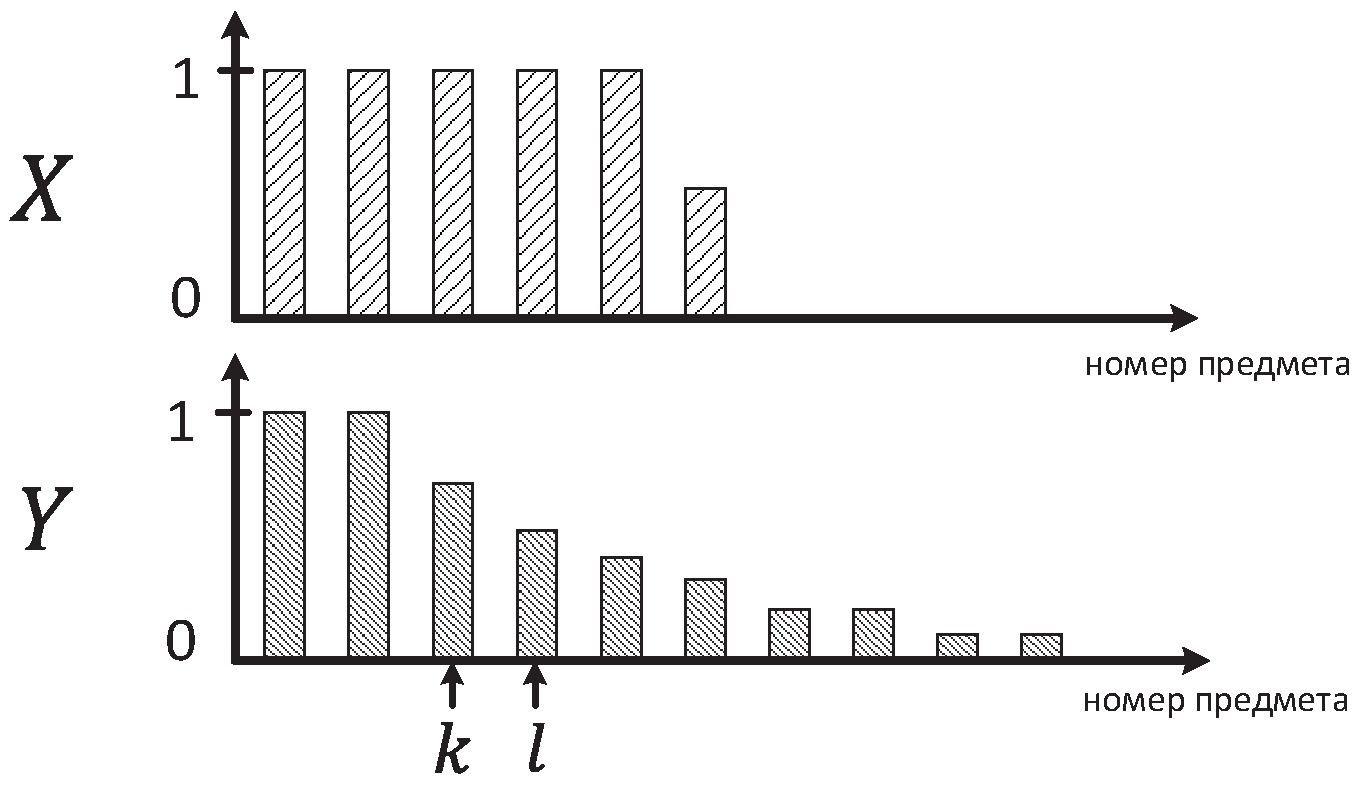
\includegraphics[width=0.6\textwidth]{Chapter3/X_Y.pdf}
\caption{Вид решений $X$ и $Y$}
\label{fig:X_Y_Solutions}
\end{center}
\end{figure}

Покажем, каким образом возможно перераспределить доли взятых предметов $y_k$ и $y_l$ под индексами $k$ и $l$ соответственно, для максимизации целевой функции системы (\ref{eq:fksp_general}).

Для этого введем следующие обозначения:
\begin{itemize}
	\item $w_{s}$~--~суммарный вес взятых предметов $k$ и $l$: $$w_{s} = y_k w_k + y_l w_l.$$ Так как значение $y_k < 1$ и $y_l \in (0, 1]$, то $w_{s} < w_k + w_l$.
	\item Обновленное решение $Y^{*}$: $$Y^{*}=(y_1, \ldots, y_{k-1}, y_k^{*}, y_{k+1}, \ldots, y_{l-1}, y_l^{*}, y_{l+1}, \ldots),$$ где $y_k^{*}$ и $y_l^{*}$~--~обновленные доли предметов под индексами $k$ и $l$ соответственно.
\end{itemize}

Решения $Y$ и $Y^{*}$ удовлетворяют ограничениям оптимизационной задачи (\ref{eq:fksp_general}) и отличаются только в долях предметов под индексами $k$ и $l$. В настоящем доказательстве, будет показано, что за счет преобразования долей $y_k$ и $y_l$ (решение $Y$) в $y_k^{*}$ и $y_l^{*}$ (решение $Y^{*}$) соответственно, без изменения остальных значений долей предметов возможно увеличить значение целевой функции задачи (\ref{eq:fksp_general}). Будет показано, что для любого решения $Y$ найдется решение $Y^{*}$, отличное в позициях $k$ и $l$, такое что целевая функция при решении $Y^{*}$ больше, чем при $Y$, что приводит к противоречию.

Для этого поставим промежуточную оптимизационную задачу:
\begin{equation}
\begin{array}{l}
\text{ \textbf{Максимизировать:} } f(y_k^{*}) + f(y_l^{*}) \\
\text{ \textbf{При условии:} }\\
\begin{cases}
w_{s} = y_k^{*} w_k + y_l^{*} w_l \\
w_s < w_k + w_l \\
w_k < w_l \\
y_k^{*},y_l^{*} \in [0,1]
\end{cases}
\end{array}.
\label{eq:inter_proof_fksp_lemma}
\end{equation}

В промежуточной оптимизационной задаче (\ref{eq:inter_proof_fksp_lemma}) целевая функция состоит из суммы функций $f(\cdot)$ для долей предметов $k$ и $l$, так как решение $Y^{*}$ отлично от $Y$ только в данных позициях. Значения остальных элементов суммы являются константами и не влияют на значение целевой функции. В ограничениях задачи (\ref{eq:inter_proof_fksp_lemma}) указывается, что суммарный вес предметов $k$ и $l$ не может быть изменен, а значит не будет нарушено ограничение на суммарный вес всех предметов взятых в рюкзак в системе (\ref{eq:fksp_general}).

Таким образом, целью промежуточной оптимизационной задачи (\ref{eq:inter_proof_fksp_lemma}) является отыскание таких $y_k^{*}$ и $y_l^{*}$, при которых целевая функция задачи (\ref{eq:inter_proof_fksp_lemma}) принимает максимальное значение. Важно отметить, что максимизация целевой функции промежуточной задачи (\ref{eq:inter_proof_fksp_lemma}) приводит и к максимизации целевой функции в обобщенной непрерывной задаче о рюкзаке (\ref{eq:fksp_general}). Как следствие, если решение $Y$ может быть улучшено в промежуточной оптимизационной задаче, то оно не является оптимальным решением задачи (\ref{eq:fksp_general}).

Продолжим рассмотрение промежуточной оптимизационной задачи. Из системы (\ref{eq:inter_proof_fksp_lemma}) выразим $y_k^{*}$ как функцию от $y_l^{*}$:
$$y_k^{*} = \frac{w_s - y_l^{*} w_l}{w_k}.$$

Подставим полученный результат в систему (\ref{eq:inter_proof_fksp_lemma}):

\begin{equation}
\begin{array}{l}
\text{ \textbf{Максимизировать:} } f\left(\frac{w_s - y_l^{*} w_l}{w_k}\right) + f(y_l^{*}) \\
\text{ \textbf{При условии:} }\\
\begin{cases}
y_k^{*} = \frac{w_s - y_l^{*} w_l}{w_k}\\
w_s < w_k + w_l \\
w_k < w_l \\
y_k^{*},y_l^{*} \in [0,1]
\end{cases}
\end{array}.
\label{eq:inter_proof_fksp_lemma_upd}
\end{equation}

Найдем вторую производную целевой функции задачи (\ref{eq:inter_proof_fksp_lemma_upd}):
$$\left[f\left(\frac{w_s - y_l^{*} w_l}{w_k}\right) + f(y_l^{*})\right]'' = f''\left(\frac{w_s - y_l^{*} w_l}{w_k}\right) \left(\frac{w_l}{w_k}\right)^2 + f''(y_l^{*}).$$

Так как функция $f(x)$ является выпуклой вниз, то $f''(x) > 0$. Следовательно, выражение в правой части является положительным, и экстремумом оптимизационной задачи (\ref{eq:inter_proof_fksp_lemma_upd}), если он существует, является минимум. Как следствие, максимальное значение целевой функции достигается на граничных значениях $y_l^{*}$ (рисунок~\ref{fig:ObjectiveFunctions}).

\begin{figure}[htbp]
\begin{center}
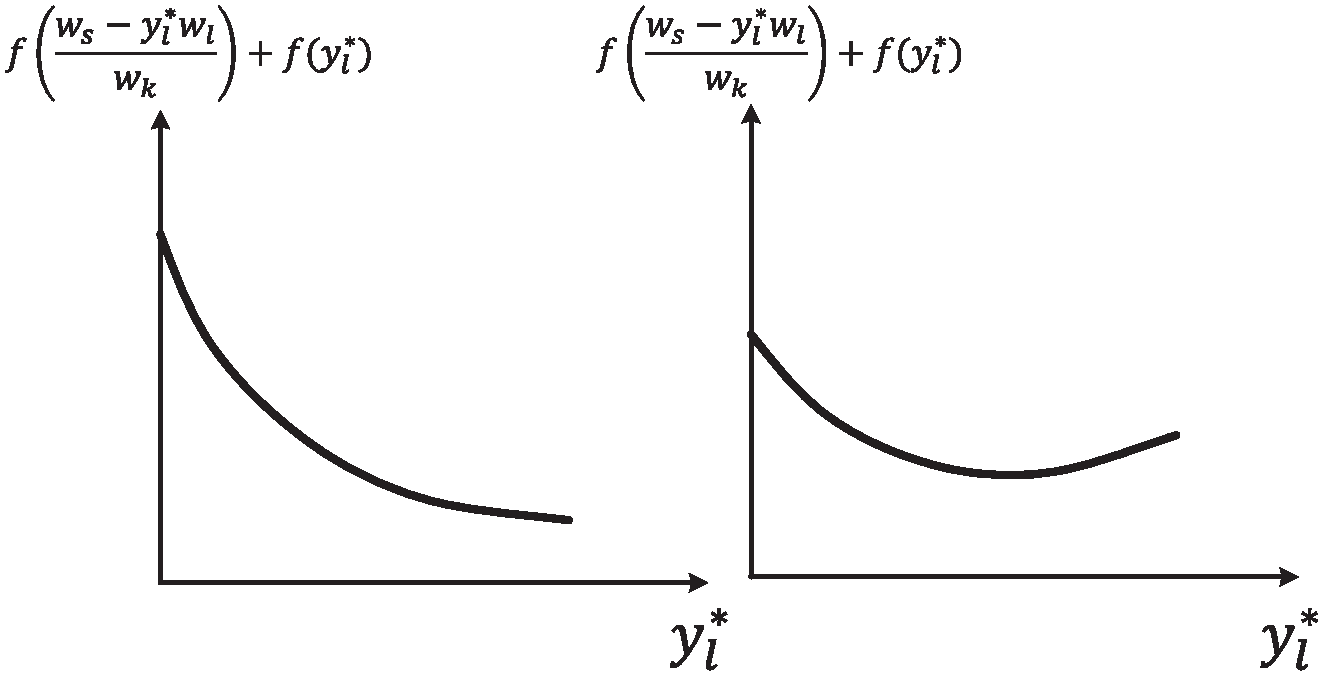
\includegraphics[width=0.8\textwidth]{Chapter3/objective_fuctions.pdf}
\caption{Вид целевой функции промежуточной оптимизационной задачи}
\label{fig:ObjectiveFunctions}
\end{center}
\end{figure}

Воспользуемся методом последовательного анализа вариантов для значения $w_s$ \cite{optimizations_methods}: разобьем все возможные значения $w_s$ на три интервала (рисунок \ref{fig:line}):
\begin{itemize}
	\item $I$: $w_s \in (0, w_k]$;
	\item $II$ : $w_s \in (w_k, w_l]$;
	\item $III$ : $w_s \in (w_l, w_k+w_l)$.
\end{itemize}

\begin{figure}[h!]
\begin{center}
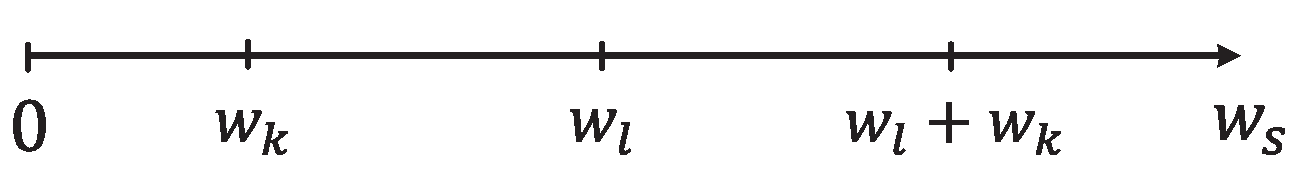
\includegraphics[width=0.7\textwidth]{Chapter3/line.pdf}
\caption{Возможные значения $w_s$}
\label{fig:line}
\end{center}
\end{figure}

Для каждого перечисленного выше интервала построим граничные значения целевой функции (\ref{eq:inter_proof_fksp_lemma_upd}).

\textbf{\textit{Интервал $I$}:}

Построим граничные значения для целевой функции оптимизационной задачи (\ref{eq:inter_proof_fksp_lemma_upd}), при $w_s \in (0, w_k]$. Для этого необходимо соблюсти все ограничения оптимизационной задачи. Важным ограничением является условие $y_k^{*},y_l^{*} \in [0,1]$. Для обеспечения $y_k^{*} \geq 0$ необходимо, чтобы значение $y_l^{*}$ не превышало $\frac{w_s}{w_l}$. Ограниченность значения $w_s$ величиной $w_k$ приводит к невозможности превышения значениями $y_l^{*}$ и $y_k^{*}$ единицы.

Основываясь на данных рассуждениях, $y_l^{*}$ может принимать значения на отрезке $\left[0, \frac{w_s}{w_l}\right]$, и граничные значения могут быть представлены следующим образом:
\begin{itemize}
	\item Граничное значение \textit{$I$.1}:
		$$\begin{cases}
		y_k^{*} = \frac{w_s}{w_k}\\
		y_l^{*} = 0
		\end{cases}.$$
		Значение целевой функции: $f\left(\frac{w_s}{w_k}\right) + f(0)$;
	\item Граничное значение \textit{$I$.2}:
		$$\begin{cases}
		y_k^{*} = 0\\
		y_l^{*} = \frac{w_s}{w_l}
		\end{cases}.$$
		Значение целевой функции: $f(0) + f\left(\frac{w_s}{w_l}\right)$.
\end{itemize}

На основании фактов что функция $f(x)$ является монотонно возрастающей и $w_k < w_l$ следует, что $f\left(\frac{w_s}{w_k}\right) > f\left(\frac{w_s}{w_l}\right)$, так как $\frac{w_s}{w_k} > \frac{w_s}{w_l}$. Следовательно, граничное значение \textit{$I$.1} максимизирует целевую функцию на интервале $I$.

\textbf{\textit{Интервал $II$}:}

На интервале, когда $w_s \in (w_k, w_l]$ важно ограничить сверху значение $y_k^{*}$ единицей, для этого величина $y_l^{*}$ должна превышать $\frac{w_s - w_k}{w_l}$. Неотрицательность $y_k^{*}$ обеспечивается ограниченностью сверху $y_l^{*}$ величиной $\frac{w_s}{w_l}$. Из $w_s \leq w_l$ следует, что $y_l^{*} \leq 1$.

Основываясь на данных рассуждениях, $y_l^{*}$ может принимать значения на отрезке $\left[\frac{w_s - w_k}{w_l}, \frac{w_s}{w_l}\right]$, и граничные значения могут быть представлены следующим образом:

\begin{itemize}
	\item Граничное значение \textit{$II$.1}:
		$$\begin{cases}
		y_k^{*} = 1 \\
		y_l^{*} = \frac{w_s - w_k}{w_l}
		\end{cases}.$$
		Значение целевой функции: $f(1) + f\left(\frac{w_s - w_k}{w_l}\right)$;
	\item Граничное значение \textit{$II$.2}:
		$$\begin{cases}
		y_k^{*} = 0\\
		y_l^{*} = \frac{w_s}{w_l} \leq 1
		\end{cases}.$$
		Значение целевой функции: $f(0) + f\left(\frac{w_s}{w_l}\right) \leq f(0) + f(1)$.
\end{itemize}

Очевидно, что граничное значение \textit{$II$.1} максимизирует целевую функцию на интервале $II$.

\textbf{\textit{Интервал $III$}:}

На интервале $w_s \in (w_l, w_k+w_l)$ проведя рассуждения, аналогичные представленным ранее, $y_l^{*}$ может принимать значения на отрезке $\left[\frac{w_s - w_k}{w_l}, 1\right]$ для выполнения всех ограничений оптимизационной задачи (\ref{eq:inter_proof_fksp_lemma_upd}). Граничные значения могут быть представлены следующим образом:
\begin{itemize}
	\item Граничное значение \textit{$III$.1}:
		$$\begin{cases}
		y_k^{*} = 1 \\
		y_l^{*} = \frac{w_s - w_k}{w_l}
		\end{cases}.$$
		Значение целевой функции: $f(1) + f\left(\frac{w_s - w_k}{w_l}\right)$;
	\item Граничное значение \textit{$III$.2}:
		$$\begin{cases}
		y_k^{*} = \frac{w_s - w_l}{w_k}\\
		y_l^{*} = 1
		\end{cases}.$$
		Значение целевой функции: $f\left(\frac{w_s - w_l}{w_l}\right) + f(1)$.
\end{itemize}

Не составляет трудностей показать, что $\frac{w_s - w_k}{w_l} > \frac{w_s - w_l}{w_k}$, основываясь на следующих неравенствах: $w_s < w_k + w_l$ и $w_k < w_l$. Следовательно, граничное значение \textit{$III$.1} максимизирует целевую функцию на интервале $III$.

Таким образом, решение оптимизационной задачи (\ref{eq:inter_proof_fksp_lemma}) задается таблицей \ref{tab:inter_proof_fksp_lemma_solution}. Таблица \ref{tab:inter_proof_fksp_lemma_solution} организована следующим образом: по заданному значению $w_s$ определяются оптимальные значения $y_k^{*}$ и $y_l^{*}$.

\begin{table}[!h]
    \caption{Решение промежуточной оптимизационной задачи}
    \begin{center}
		\label{tab:inter_proof_fksp_lemma_solution}
	    \begin{tabular}{| C{4cm} | C{4cm} | C{4cm} |}
	    	\hline
	    	Значение $w_s$ & Оптимальное значение $y_k^{*}$  & Оптимальное значение $y_l^{*}$ \\
	    	\hline
			$(0, w_k]$ & $$\frac{w_s}{w_k}$$ & $$0$$\\
	    	\hline
			$(w_k, w_k+w_l]$ & $$1$$ & $$\frac{w_s - w_k}{w_l}$$\\
	    	\hline
    	\end{tabular}
	\end{center}
\end{table}

При всех возможных значениях $w_s$ перераспределение долей взятых предметов в пользу предмета $k$ за счет всей взятой доли предмета $l$ приводит к максимизации целевой функции оптимизационной задачи (\ref{eq:inter_proof_fksp_lemma}) (таблица \ref{tab:inter_proof_fksp_lemma_solution}). Следовательно, решение $Y$ возможно улучшить за счет перераспределения долей предметов под индексами $k$ и $l$. Вид решений $X$, $Y$ и $Y^{*}$ представлен на рисунке \ref{fig:X_Y_Ys_Solutions}.

\begin{figure}[htbp]
\begin{center}
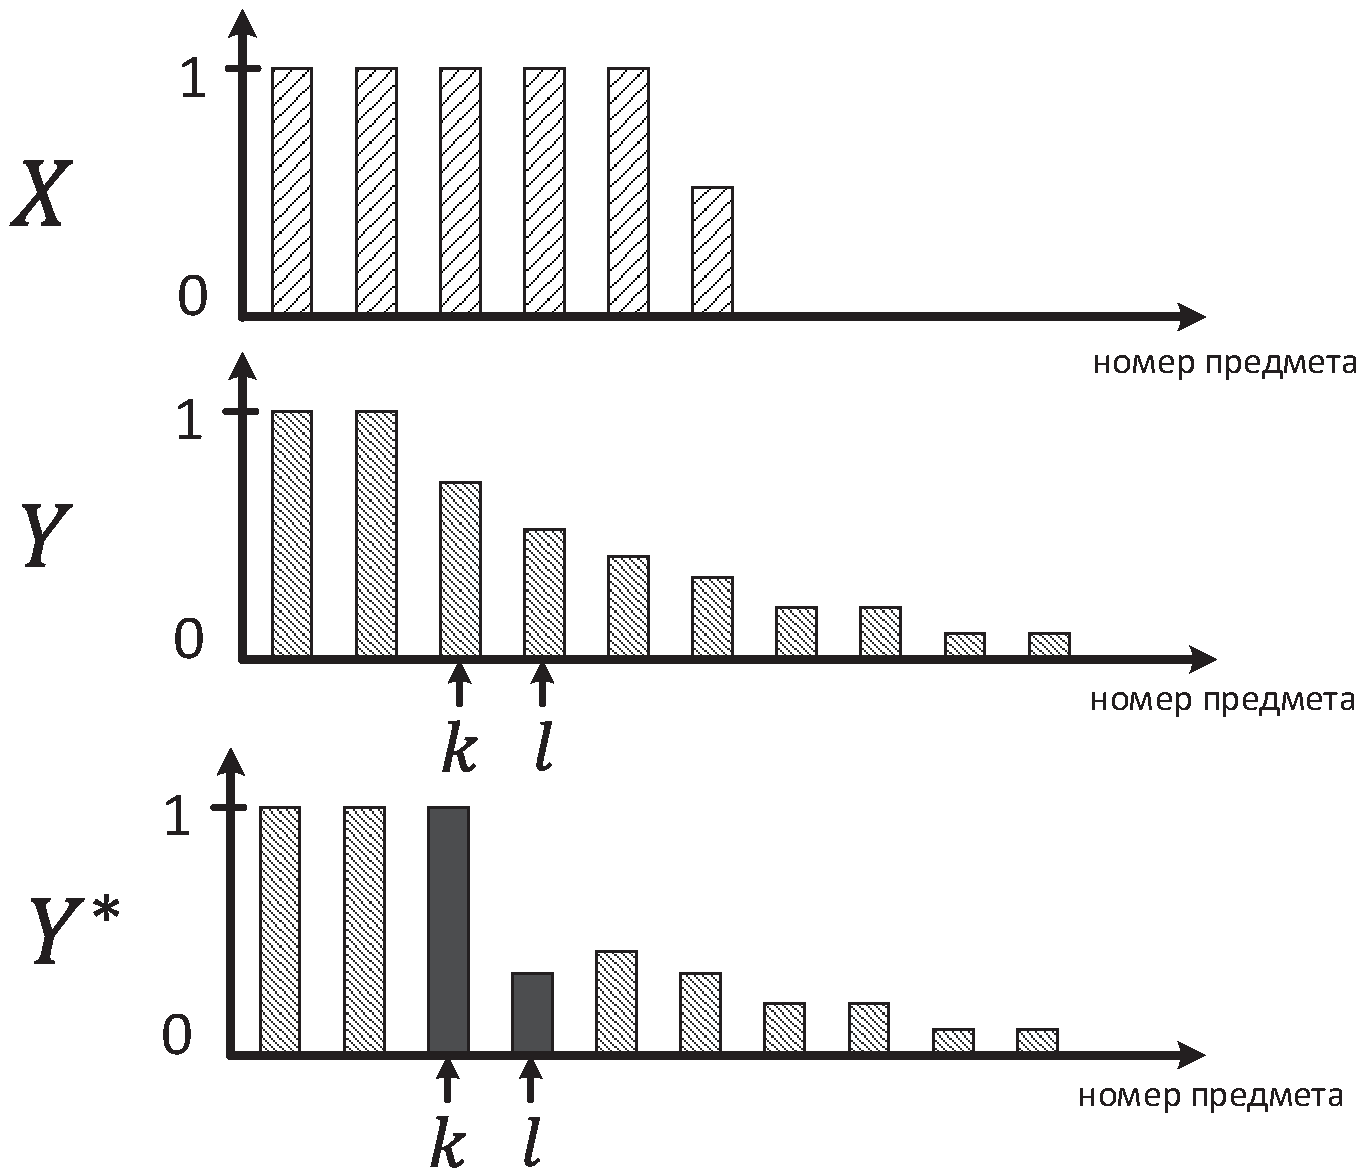
\includegraphics[width=0.6\textwidth]{Chapter3/X_Y_Z.pdf}
\caption{Вид решений $X$, $Y$ и $Y^{*}$}
\label{fig:X_Y_Ys_Solutions}
\end{center}
\end{figure}

Таким образом, любое решение $Y$, в котором найдутся предметы с индексами $k$ и $l$ может быть улучшено до решения $Y^{*}$, значение целевой функции которой больше, чем у $Y$. Большее значение целевой функции при решении $Y^{*}$, по сравнению с $Y$, обеспечивается тем, что $Y^{*}$ является решением промежуточной оптимизационной задачи (\ref{eq:inter_proof_fksp_lemma}).

Следовательно, всевозможные решения $Y$ не являются оптимальными для обобщенной непрерывной задачи о рюкзаке (\ref{eq:fksp_general}), что является противоречием. Одновременно с этим важно отметить, что для решения $X$, полученного алгоритмом \ref{alg:algorithm_lemma}, не найдется пары предметов с индексами $k$ и $l$, следовательно оно не может быть улучшено и является оптимальным для оптимизационной задачи (\ref{eq:fksp_general}).
\end{proof}

Проведем анализ сложности предложенного решения непрерывной задачи о рюкзаке. Для этого рассмотрим каждый шаг алгоритма \ref{alg:algorithm_lemma}:
\begin{itemize}
	\item Шаг 1. Сортировка пользователей в порядке возрастания отношений $\frac{w_i}{c_i}$. Сложность данного шага составляет $O(N \log_2 N), N\to\infty$ при использовании быстрой сортировки;
	\item Шаг 2. Поиск предмета с индексом $j$ может быть осуществлен с линейной сложностью: $O(N), N\to\infty$;
	\item Шаг 3. Вычисление оптимальных значений $x_i, i=\overline{1,N}$ может быть реализовано с линейной сложностью: $O(N), N\to\infty$.
\end{itemize}
Сложность алгоритма \ref{alg:algorithm_lemma} определяется Шагом 1 и равняется $O(N \log_2 N), N\to\infty$.

Для непрерывных задач выпуклого программирования от нескольких переменных с ограничениями типа равенств и неравенств существуют несколько методов отыскания экстремумов \cite{convex_opt,optimizations_methods}:
\begin{itemize}
	\item Получение замкнутого выражения для экстремума на основе условий Каруша-Куна-Таккера (ККТ);
	\item Получение численного решения на основе условий ККТ;
	\item Численные методы нелинейного программирования.
\end{itemize}

Стандартным методом решения задач выпуклого программирования является поиск решения удовлетворяющих условиям Каруша-Куна-Таккера \cite{convex_opt,optimizations_methods}. Данный метод сводится к нахождению решения системы нелинейных уравнений и неравенств. В результате решения данной системы может быть получено замкнутое выражение для условного экстремума. Тогда сложность полученного решения заключается в вычислении значений по заданным входным данным. Сложность вычисления решения растет линейно от числа переменных $N$: $O(N), N\to\infty$.

Однако, ввиду большого числа переменных в системе, полученной на основе условий ККТ, получение замкнутого решения может быть затруднительно. Для решения подобных систем может быть применен метод, известный в англоязычной литературе как \textit{<<water-filling>>}, подробно описанный в \cite{convex_opt}. Данный метод позволяет найти решение системы с использованием численной процедуры. В настоящей работе, метод \textit{<<water-filling>>} был применен для решения оптимизационной задачи, представленной в подразделе \ref{chap4:KktSolution}. Сложность вычисления решения определяется сложностью процедуры получения численного решения.

Для решения задач выпуклого программирования от нескольких переменных с ограничениями типа равенств и неравенств известны численные методы: методы спуска и штрафных функций \cite{optimizations_methods}. Важно отметить, что для задач выпуклого программирования данные методы сходятся к оптимальному решению, так как в подобных задачах существует только один экстремум. Оценить сложность получения решения оптимизационных задач с использованием подобных методов не представляется возможным, так как данные методы являются итеративными и зависят от начальных значений поиска экстремума (невозможно предсказать число шагов, необходимых для нахождения оптимальных значений оптимизационной задачи). Сравнение сложности методов решения оптимизационных задач выпуклого программирования от нескольких переменных с ограничениями типа равенств и неравенств представлены в таблице~\ref{tab:nonadaptiveComplexity}.

\begin{table}[!h]
    \caption{Сравнение сложности методов решения обобщенной непрерывной задачи о рюкзаке}
    \begin{center}
		\label{tab:nonadaptiveComplexity}
	    \begin{tabular}{| C{5cm} | C{5cm} | C{5cm} |}
	    	\hline
	    	Название метода & Характеристика сложности метода при наличии $N$ переменных & Возможность реализации в реальном масштабе времени\\
	    	\hline
			Замкнутое выражение (ККТ) & $$O(N), N\to\infty$$ & $$+$$\\
	    	\hline
			Решение на основе алгоритма \ref{alg:algorithm_lemma} & $$O(N \log_2 N), N\to\infty$$ & $$+$$\\
	    	\hline
	    	Численное решение системы условий ККТ & Зависит от процедуры получения численного решения & $$+/-$$ \\
	    	\hline
	    	Численные методы нелинейного программирования & Высокая сложность & $$-$$ \\
	    	\hline
    	\end{tabular}
	\end{center}
\end{table}

Таким образом, при сравнении сложности полученного решения на основе алгоритма \ref{alg:algorithm_lemma} со стандартными методами решения непрерывных задач выпуклого программирования от нескольких переменных с ограничениями типа равенств и неравенств справедливо следующее утверждение: \textit{сложность решения на основе алгоритма \ref{alg:algorithm_lemma} является приемлемой в сравнении со стандартными методами решения подобных задач}.

Решение оптимизационной задачи (\ref{eq:fksp_general}) алгоритмом \ref{alg:algorithm_lemma} может быть вычислено в режиме реального времени. Под режимом реального времени понимается возможность вычисления оптимальных значений в короткий промежуток времени. В настоящей работе за единицу времени принят интервал планирования равный $1$ мс (подраздел~\ref{chap2:RadioChannel}). Элементарно показывается, что на современных процессорах алгоритм \ref{alg:algorithm_lemma} может быть выполнен за промежуток времени не превышающий интервал планирования.

\section{Нижняя граница нормированного отношения длительностей буферизации и просмотра при передаче неадаптивных видеопотоков}
\label{chap3:LowerBoundForG}

В подразделе \ref{chap3:NonAdaptiveOptimizationProblem} была поставлена оптимизационная задача нелинейного программирования (\ref{eq:optim_problem_g}), решение которой определяет нижнюю границу для среднего значения нормированного отношения длительностей буферизации и просмотра $G$ (определение~\ref{def:gMetric}) по множеству всех возможных алгоритмов планирования $\mathcal{A}$, удовлетворяющих введенных ограничениям в подразделе \ref{chap2:Assumptions}. В подразделе \ref{chap3:GeneralizedFKSP} была представлена обобщенная непрерывная задача о рюкзаке, когда в целевой функции фигурирует сумма выпуклых функций, и предложен алгоритм нахождения решения данной задачи, с низкой вычислительной сложностью. Настоящий подраздел ставит своей задачей найти нижнюю границу для критерия качества $G$, основываясь на результатах, полученных в подразделе \ref{chap3:GeneralizedFKSP}.

Оптимизационная задача (\ref{eq:optim_problem_g}) имеет следующий вид:
\begin{equation}
\nonumber
\begin{array}{l}
\text{ \textbf{Минимизировать:} } G = \sum\limits_{i=1}^{N} {g_i} \\
\text{ \textbf{При условии:} }\\
\begin{cases}
\sum\limits_{i=1}^{N} {\frac{K_i (1-g_i)}{g_i + \gamma (1-g_i)}} \leq 1 \\
g_i \in [0,1], i=\overline{1,N}
\end{cases}
\end{array},
\end{equation}
где $K_i=R_i E[C_i^{-1}]$, $\gamma$~--~коэффициент разреженности видеопотока (определение \ref{def:VideoSparseness}).

\begin{theoremapp}
\label{thr:GTheorem}
Решение задачи нелинейного программирования (\ref{eq:optim_problem_g}), характеризующее нижнюю границу нормированного отношения длительностей буферизации и просмотра при передаче неадаптивных видеопотоков, может быть получено алгоритмом \ref{alg:GTheoremAlgorithm}.
\end{theoremapp}

\begin{algorithm}
  \caption{: Решение задачи (\ref{eq:optim_problem_g})}
	\label{alg:GTheoremAlgorithm}
  \begin{algorithmic}[1]
	 \item Сортировка пользователей по возрастанию отношений $\frac{K_i}{\gamma}$, и их нумерация, в соответствие с сортировкой;
	 \item Нахождение пользователя с индексом $j:\begin{cases}
		\sum\limits_{i=1}^{j-1} {\frac{K_i}{\gamma}} \leq 1 \\
		\sum\limits_{i=1}^{j} {\frac{K_i}{\gamma}} > 1
		\end{cases}$
		\newline
		если $j\in\varnothing$, то $j=N+1$;
	\item Нахождение оптимальных значений $g_i$: \newline
	$g_i=\begin{cases}
		0, & i < j \\
		\frac{\gamma (1 - \xi)}{\xi + \gamma (1-\xi)}, & i=j \\
		1, & i > j
		\end{cases}$,\newline
		где $\xi = \frac{\gamma}{K_j}\left(1 - \sum\limits_{i=1}^{j-1} {\frac{K_i}{\gamma}}\right)$.
  \end{algorithmic}
\end{algorithm}

\begin{proof}

Для доказательства теоремы \ref{thr:GTheorem} произведем несколько преобразований системы (\ref{eq:optim_problem_g}).

Вынесем из знаменателя нелинейного ограничения $\gamma$:

$$\sum\limits_{i=1}^{N} {\frac{K_i (1-g_i)}{g_i + \gamma (1-g_i)}} = \sum\limits_{i=1}^{N} \left(\frac{K_i}{\gamma}\right) {\frac{(1-g_i)}{\frac{g_i}{\gamma} + (1-g_i)}}.$$

Преобразуем задачу (\ref{eq:optim_problem_g}) из задачи минимизации в задачу максимизации:

\begin{equation}
\nonumber
\label{eq:GTheorem_1}
\begin{array}{l}
\text{ \textbf{Максимизировать:} } \sum\limits_{i=1}^{N} {(1-g_i)} \\
\text{ \textbf{При условии:} }\\
\begin{cases}
\sum\limits_{i=1}^{N} \left(\frac{K_i}{\gamma}\right) {\frac{(1-g_i)}{\frac{g_i}{\gamma} + (1-g_i)}} \leq 1 \\
g_i \in [0,1], i=\overline{1,N}
\end{cases}
\end{array}.
\end{equation}

Введем обозначение:
$$x_i = \frac{(1-g_i)}{\frac{g_i}{\gamma} + (1-g_i)}.$$
Значение $x_i$ монотонно зависит от величины $g_i$ и может принимать значения в отрезке $[0,1]$. Выразим значения $g_i$ и $(1-g_i)$ из $x_i$:
\begin{equation}
\label{eq:GTheorem_interrelation}
g_i = \frac{\gamma (1 - x_i)}{x_i + \gamma (1-x_i)},
\end{equation}
$$1-g_i = \frac{x_i}{x_i + \gamma (1-x_i)}.$$

При введенных обозначениях оптимизационная задача (\ref{eq:optim_problem_g}) принимает следующий вид:
\begin{equation}
\label{eq:GTheorem_2}
\begin{array}{l}
\text{ \textbf{Максимизировать:} } \sum\limits_{i=1}^{N} {\frac{x_i}{x_i + \gamma (1-x_i)}} \\
\text{ \textbf{При условии:} }\\
\begin{cases}
\sum\limits_{i=1}^{N} \left(\frac{K_i}{\gamma}\right) {x_i} \leq 1 \\
x_i \in [0,1], i=\overline{1,N}
\end{cases}
\end{array}.
\end{equation}

Проведем анализ целевой функции оптимизационной задачи (\ref{eq:GTheorem_2}) и покажем, что данная целевая функция соответствует требованиям, налагаемыми на целевую функцию оптимизационной задачи (\ref{eq:fksp_general}). Из вида функции очевидно, что она непрерывна, строго монотонно возрастает и ограничена сверху и снизу на области определения $x_i$. Проведем анализ второй производной:
$$\left[\frac{x_i}{x_i + \gamma (1-x_i)}\right]'' = \frac{2\gamma(\gamma - 1)}{(x_i + \gamma(1 - x_i))^3}.$$
По определению значение $\gamma \geq 1$, так же величина $x_i$, по условию оптимизационной задачи, может принимать значения в отрезке $[0,1]$, следовательно вторая производная неотрицательна в области определения $x_i$.

Основываясь на представленном анализе, $\frac{x_i}{x_i + \gamma (1-x_i)}$~--~непрерывная, выпуклая вниз функция, дважды дифференцируемая, строго монотонно возрастающая и ограниченная на области определения $x_i$ функция. Исходя из описанного выше и результатов, представленных в подразделе \ref{chap3:GeneralizedFKSP}, справедливо следующее утверждение: решение задачи (\ref{eq:GTheorem_2}) может быть получено при использовании алгоритма \ref{alg:algorithm_lemma}, где $w_i = \left(\frac{K_i}{\gamma}\right), c_i = 1, i=\overline{1,N}$ и $W = 1$.

Алгоритм \ref{alg:GTheoremAlgorithm} является адаптацией алгоритма \ref{alg:algorithm_lemma} в обозначениях оптимизационной задачи (\ref{eq:optim_problem_g}) и взаимосвязи между значениями $g_i$ и $x_i$ (выражение \ref{eq:GTheorem_interrelation}). Данный факт завершает доказательство.
\end{proof}

Решением задачи (\ref{eq:optim_problem_g}) является вектор отношений длительностей буферизации и просмотра для каждого пользователя: $(g_1, g_2, \ldots, g_N)$, обладающий минимально возможной суммой элементов, удовлетворяющих всем ограничениям оптимизационной задачи. Среднее арифметическое элементов данного вектора является нижней границей для критерия $G$ по всем возможным алгоритмам планирования распределения ресурсов, удовлетворяющим допущениям, введенным в подразделе \ref{chap2:Assumptions}. Таким образом, в настоящем разделе была найдена граница, характеризующая максимально возможную производительность алгоритмов распределения ресурсов радиоканала в централизованных беспроводных телекоммуникационных сетях при передачи неадаптивных видеопотоков.

Настоящий результат имеет широкий спектр применения:
\begin{itemize}
	\item \textbf{Теоретическая область.} Нижняя граница может быть использована для аналитической оценки производительности централизованных беспроводных сетей для существующих и последующих стандартов беспроводной связи.
	\item \textbf{Практическая область.} Благодаря низкой вычислительной сложности расчета значений нижней границы (алгоритм \ref{alg:GTheoremAlgorithm}), настоящая нижняя граница может быть непосредственно встроена в алгоритм распределения ресурсов беспроводного канала на базовой станции. Такая возможность позволяется создать семейство алгоритмов планирования для повышения производительности сети передачи информации в целом.
\end{itemize}

Завершающая часть настоящего раздела посвящена демонстрации области практической применимости полученного результата. Далее будет предложен алгоритм планирования ресурсов беспроводного канала на базовой станции и произведено его сравнение с известными планировщиками и нижней границей.

\section{Алгоритм планирования распределения ресурсов для минимизации нормированного отношения длительностей буферизации и просмотра при передаче неадаптивных видеопотоков}
\label{chap3:NonAdaptiveScheduler}

Настоящий подраздел описывает концепцию алгоритма планирования распределения ресурсов на базовой станции, в основу которого положен результат, представленный в подразделе \ref{chap3:LowerBoundForG}. В подразделе будет предложен планировщик, опирающийся на концепцию совместного планирования ресурсов радиоканала между всеми активными пользователями в отличие от классических алгоритмов планирования (подраздел \ref{chap2:Scheduler}). Под совместным планированием подразумевается учет статистик всех активных пользователей, присутствующих в системе передачи информации в момент планирования, при распределении частотно-временных ресурсов конкретному пользователю.

Настоящий подраздел последовательно описывает этапы построения алгоритма планирования:
\begin{itemize}
	\item Определение объема доступной информации для принятия решения;
	\item Статистики и методы их вычисления;
	\item Методы управления распределением частотно-временных ресурсов;
	\item Алгоритм распределения ресурсов беспроводного канала.
\end{itemize}

Представим описание рассматриваемой системы. На рисунке~\ref{fig:PracticalModel} представлена схема беспроводной централизованной сети при передаче видеоданных, основанная на описании представленном в подразделах \ref{chap2:GeneralOverview}, \ref{chap2:RadioChannel} и \ref{chap2:Scheduler}. Важным функциональным компонентом опорной сети оператора является система анализа трафика, которая может определить тип используемого трафика и его характеристики (в англоязычной литературе данные системы известны под названием \textit{<<Deep Packet Inspection>>} или DPI).% Центральным элементом рассматриваемой схемы является планировщик базовой станции. Важным моментом в настоящем описании является объемы и моменты времени доступа к информации на основе которой алгоритм планировщика будет принимать решения распределении ресурсов беспроводного канала.

\begin{figure}[htbp]
\begin{center}
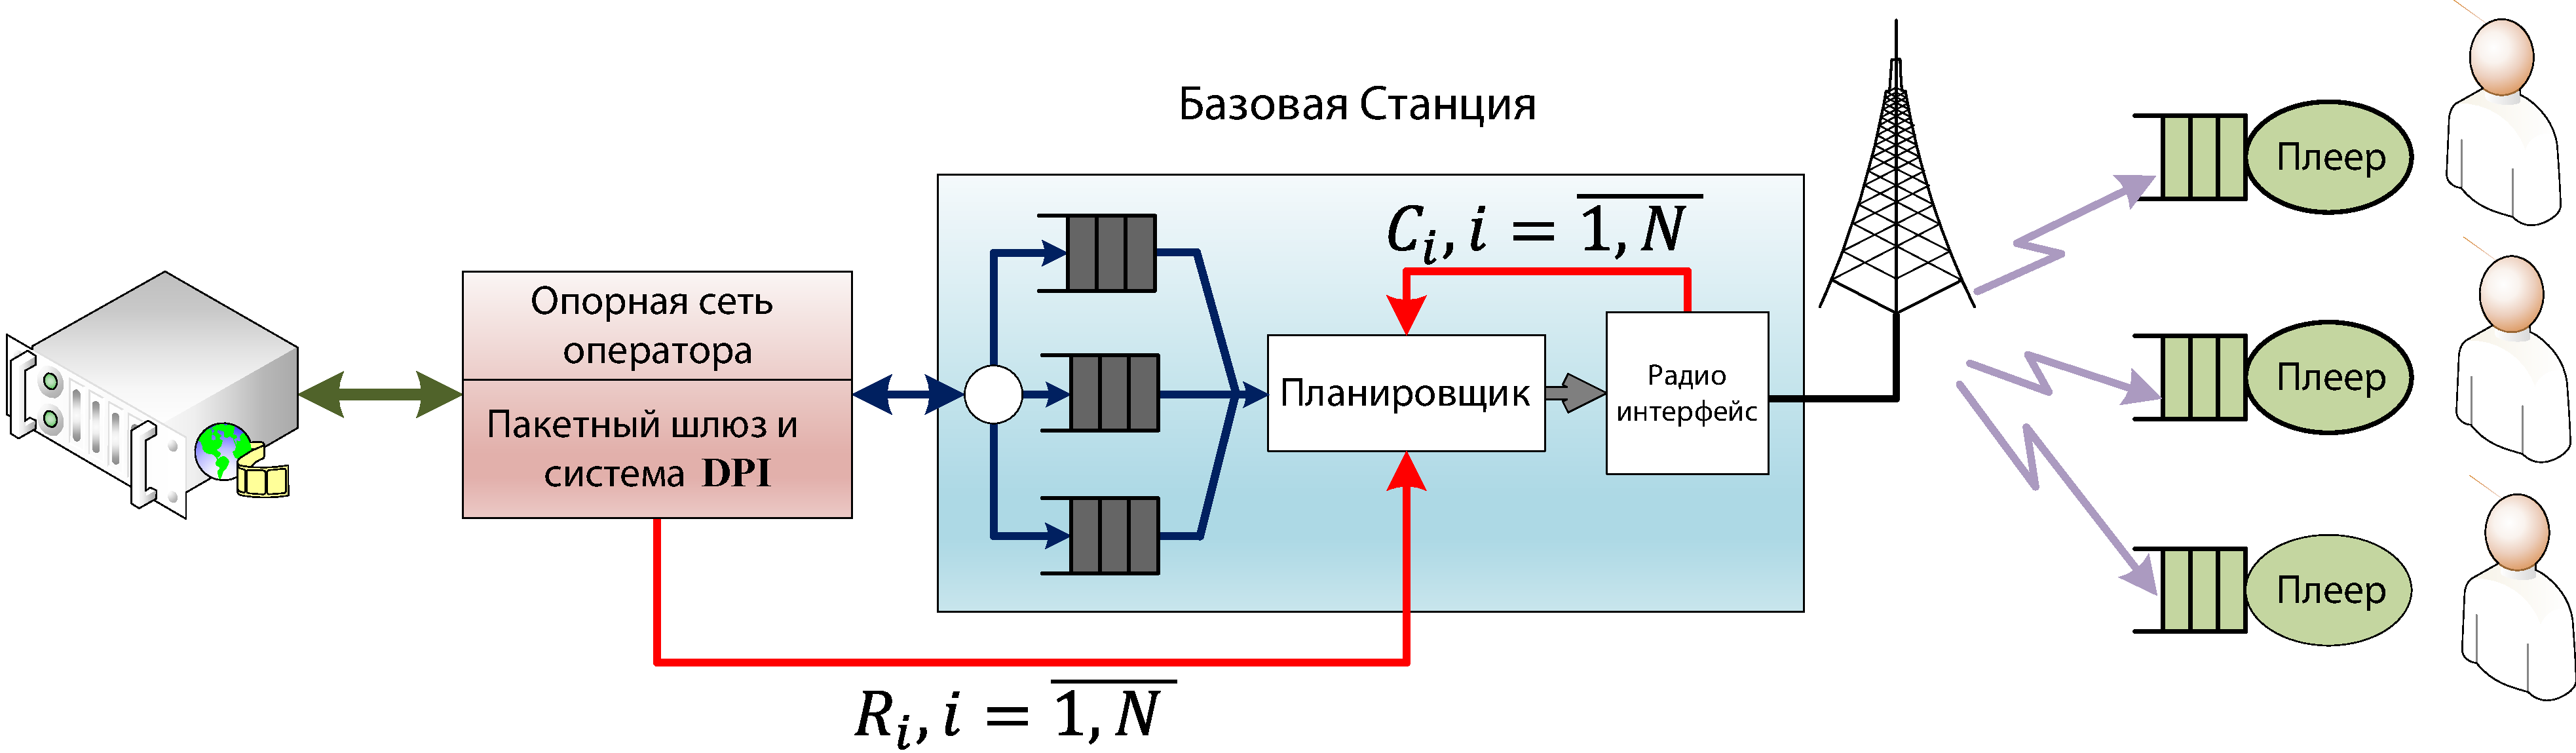
\includegraphics[width=\textwidth]{Chapter3/PracticalModel.pdf}
\caption{Концептуальная схема предлагаемого алгоритма планирования}
\label{fig:PracticalModel}
\end{center}
\end{figure}

На первом шаге описания алгоритма планирования будет представлена информация, доступная алгоритму планирования, для принятия решения. В настоящей работе, для планировщика доступна следующая информация для каждого пользователя $i$ в каждый момент времени $t$:
\begin{itemize}
	\item Битовая скорость потока $R_i(t)$, полученная от системы анализа трафика DPI;
	\item Значение максимально достижимой скорости канала $C_i(t)$, значение которой доступно от радиоинтерфейса;
	\item Объем данных доступный в очереди для передачи на пользовательское устройство $B_i(t)$;
	\item Объем переданных данных $P_i(t)$.
\end{itemize}
В существующих беспроводных централизованных системах связи время является дискретным и разбито на интервалы равной длительности $\Delta t$ секунд.

На втором шаге описания алгоритма предлагаются методы агрегирования доступной информации. Представленный ранее объем информации должен быть агрегирован в некоторые значения, называемые статистиками, которые отражают текущую ситуацию в зоне ответственности базовой станции. Наиболее критичные статистики, необходимые для функционирования планировщика, представлены следующим списком:
\begin{itemize}
	\item Активность пользователя $U_i(t)$;
	\item Оценка скорости передачи информации $S_i^{avg}(t)$;
	\item Оценка максимально достижимой скорости канала $C_i^{avg}(t)$.
\end{itemize}
Сложность вычисления данных статистик является важным параметром, налагаемым на вычислительную процедуру, ввиду жесткого временного ограничения на длительность получения результата (подраздел \ref{chap2:Scheduler}).

В настоящей работе рассматривается модель поведения пользователя, просматривающего последовательность из видеороликов (подраздел \ref{chap2:GeneralOverview}). Следовательно, пользователь может находится в двух состояниях: активном (загружает видеоданные) или неактивном (выбирает следующий ролик для просмотра). Таким образом, на уровне планировщика необходимо произвести оценку $U_i(t)$: в каком из двух состояний находится пользователь $i$ в момент времени $t$.
% Активность пользователя определяется логическим значением (истинно или ложно).
Будем считать пользователя активным, если разность между текущим моментом времени и последним моментом времени, когда у абонента $i$ были данные для передачи не превышает $t^{act}$ секунд:
\begin{equation}
	\label{eq:activityEstimation}
	U_i(t) = \mathbbm{1}\{t - t_i^{l} \leq t^{act}\},
\end{equation}
где $t_i^{l} = \max\limits_{t} \mathbbm{1}\{B_i(t) > 0\}.$

Введем обозначение $\mathcal{U}$~--~множество активных пользователей $i:U_i(t) > 0$ в момент времени $t$.

В настоящей работе рассматривается передача информации по беспроводному каналу связи, важной отличительной чертой которого является изменяемость характеристик во времени (подраздел \ref{chap2:RadioChannel}). В качестве статистики для оценок $S_i^{avg}(t)$ и $C_i^{avg}(t)$ предлагается использовать среднее значение за продолжительный промежуток времени (длительность усреднения) $\bar{w}_{S}$ и $\bar{w}_{C}$ соответственно. Ограничение интервала усреднения обусловлены изменяемостью канала связи и необходимостью поддержания актуальности статистик.

Очевидным подходом для вычисления средних значений является среднее арифметическое значение. Однако, сложность его вычисления по операциям и затрачиваемым объемом памяти достаточно высока: хранение всего массива исходных данных и его обработка. Ввиду существующих ограничений на вычислительную сложность, в качестве метода оценки предлагается использовать метод экспоненциального забывания (в литературе встречается термин <<экспоненциальное сглаживание>>):

$$X_i^{avg}(t) = \left(1 - \frac{1}{\bar{w}_{X}}\right)X_i^{avg}(t - 1) + \left(\frac{1}{\bar{w}_{X}}\right)X_i(t),$$
где $X_i(t)$~--~элемент случайного процесса, $\bar{w}_{X}$~--~длительность усреднения для процесса $X$ и $X_i^{avg}(0) = X_i(1)$.

Важной характеристикой методов оценки среднего значения за некоторый промежуток времени является скорость сходимости полученной оценки к истинному значению. На скорость сходимости среднего значения, вычисленного методом экспоненциального забывания, большое влияние оказывает длительность интервалов усреднения. Во многих случаях оценка среднего значения методом среднего арифметического и экспоненциального забывания показывает близкие значения. Однако, существует сценарий, на котором оценки, полученные по настоящим методикам, показывают разную скорость сходимости к истинному среднему значению. Подобная ситуация возможна, когда первое значение случайного процесса имеет сильное отличие от истинного среднего. Продемонстрируем это на примере: пусть существует дискретный случайный процесс $X(t) \sim N(10,1.5)$, при этом значение $X(1) = 0$, и необходимо произвести оценку его среднего значения за последние $\bar{w}_{X} = 10$ отсчетов (рисунок \ref{fig:adaptation}).

Из рисунка \ref{fig:adaptation} следует, что метод экспоненциального забывания при оценке среднего значения показывает медленную скорость сходимости к истинному среднему значению в сравнении с методом среднего арифметического. Поэтому в настоящем подразделе предлагается модифицировать метод экспоненциального забывания изменяемым во времени интервалом усреднения по следующему правилу:
$$w_{X}(t) = \min(t, \bar{w}_{X}).$$
В настоящей работе, метод оценки среднего значения, использующий изменяемый во времени интервал усреднения называется \textit{<<методом экспоненциального забывания с быстрой адаптацией>>}. Производительность данного метода оценки сравнима с методом среднего арифметического и демонстрирует достаточную скорость сходимости к истинному значению (рисунок \ref{fig:adaptation}).

\begin{figure}[htbp]
\begin{center}
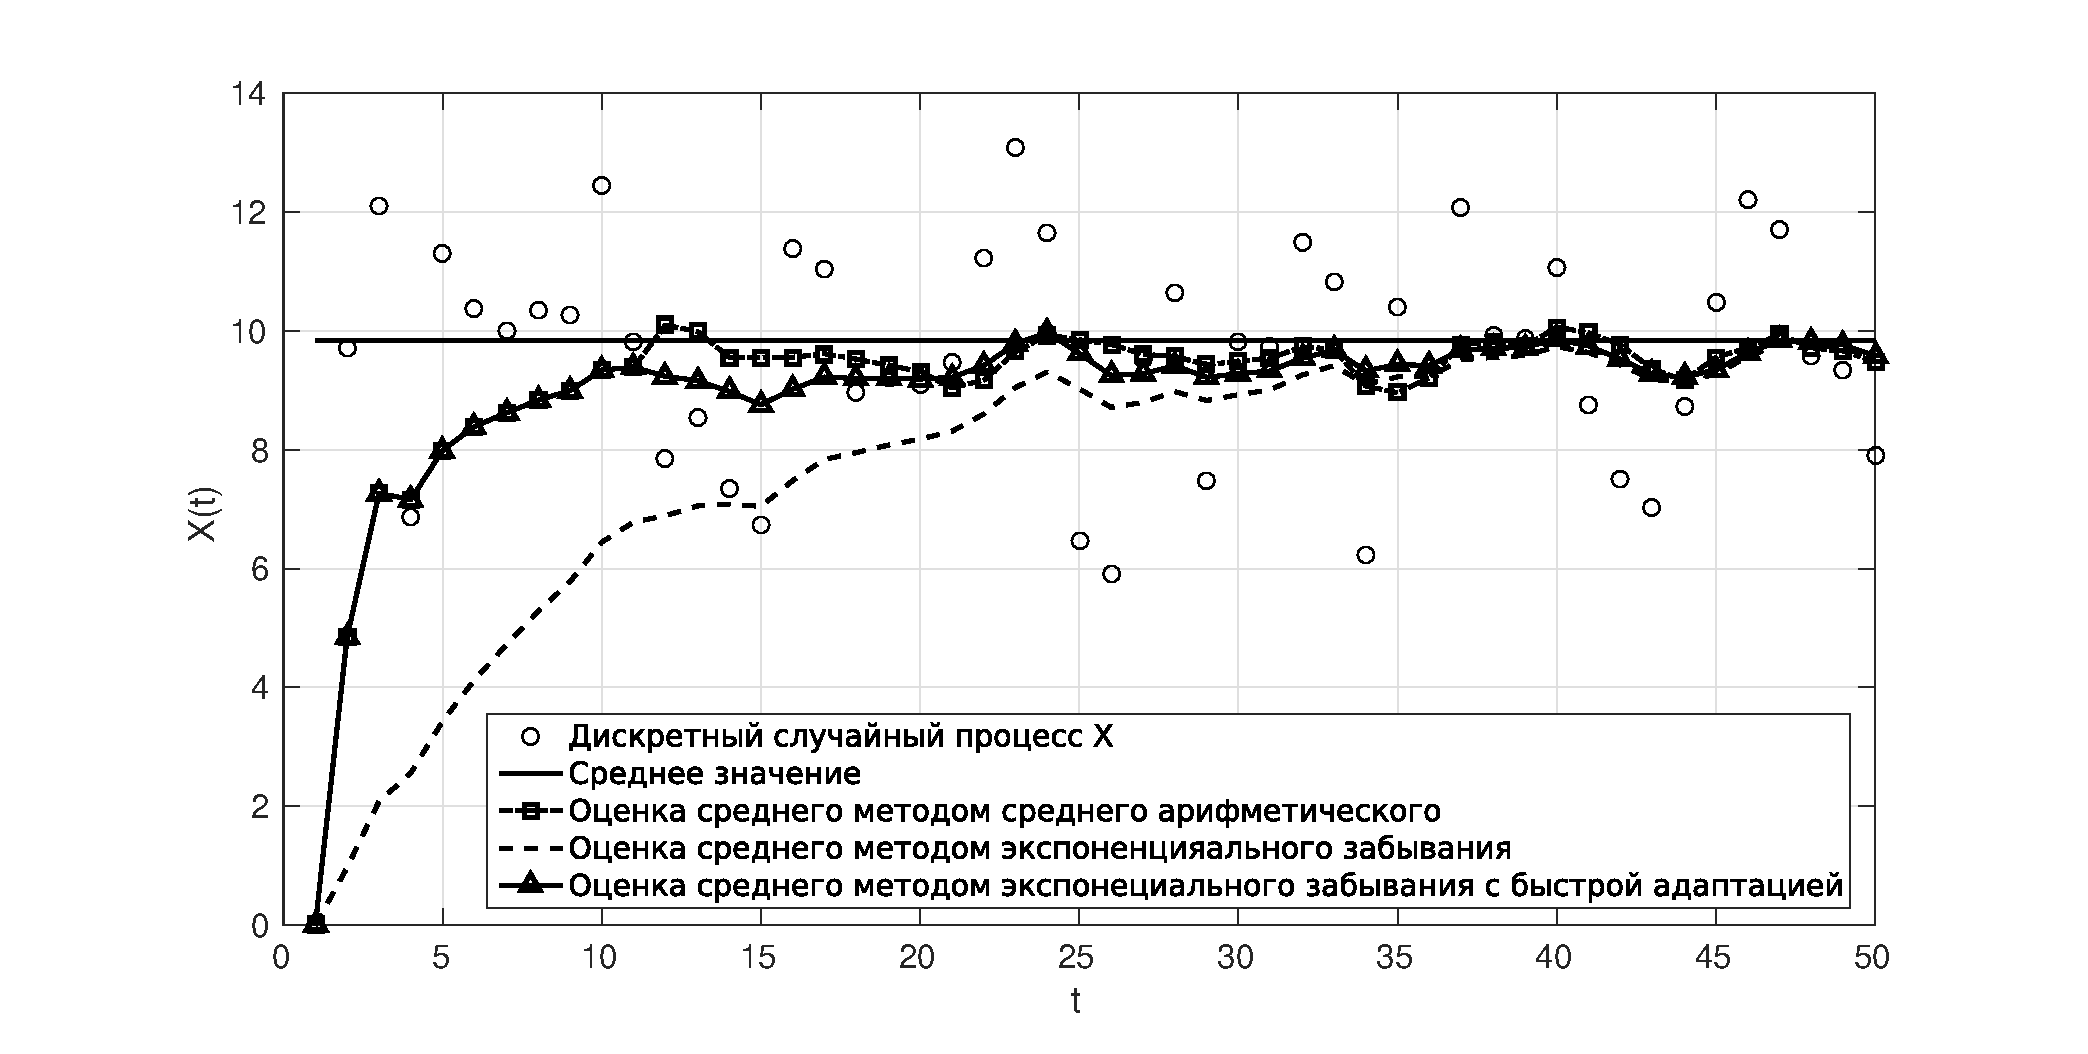
\includegraphics[width=\textwidth]{Chapter3/adaptation.eps}
\caption{Сравнение скорости сходимости методов оценки среднего значения}
\label{fig:adaptation}
\end{center}
\end{figure}

Таким образом, для оценки средних значений $C_i^{avg}(t)$ и $S_i^{avg}(t)$ предлагаются следущие методики, вычисление которых производится только при нахождении пользователя в активном состоянии:
\begin{equation}
\label{eq:CEstimation}
C_i^{avg}(t) = \left(1 - \frac{1}{w_{C}(t)}\right)C_i^{avg}(t - 1) + \left(\frac{1}{w_{C}(t)}\right)C_i(t)
\end{equation}

\begin{equation}
\label{eq:SEstimation}
S_i^{avg}(t) = \left(1 - \frac{1}{w_{S}(t)}\right)S_i^{avg}(t - 1) + \left(\frac{1}{w_{S}(t)}\right)\frac{P_i(t)}{\Delta t},\end{equation}
где $w_{C}(t) = \min (t - t_i^{l} + 1, \bar{w}_{C})$ и $w_{S}(t) = \min (t - t_i^{l} + 1, \bar{w}_{S})$  соответственно и $C_i^{avg}(0) = S_i^{avg}(0) = 0$.

Неотрицательность значений $w_{C}(t)$ и $w_{S}(t)$ обеспечивается вычислением оценок только в активном состоянии пользователя ($t - t_i^{l} \geq 0$). Подобный метод оценки поддерживает актуальность статистик, так как канал может динамично изменяться во времени, и обладает низкой вычислительной сложностью.

Следующим шагом в представлении алгоритма планирования является метод управления распределением частотно-временных ресурсов, имеющий непосредственное влияние на скорость передачи информации. Для представления данного метода необходимо описать каким образом существующие алгоритмы планирования распределяют ресурсы беспроводного канала связя. Как было описано в подразделе \ref{chap2:RadioChannel}, беспроводной канал связи разделен на ресурсные блоки, являющиеся минимальной единицей ресурсов, которая может быть выделена пользователю. Число ресурсных блоков ($N_{rb}$) в одном интервале планирования определяется шириной полосы.

В каждый момент времени $t$ для конкретного ресурсного блока $r$ вычисляется приоритет выделения для каждого пользователя $i$: $p_{r,i}(t)$. Для каждого конкретного ресурсного блока находится пользователь с максимальным приоритетом и выделяется найденному пользователю. Важно отметить, что все алгоритмы планирования не распределяют ресурсы пользователям, у которых отсутствуют данные для передачи на уровне очередей. Именно правило вычисления приоритета пользователя на ресурсный блок определяет алгоритм планирования. Наиболее известными эвристическими алгоритмами планирования являются \textit{Proportional Fair} и \textit{Round Robin}:
\begin{itemize}
	\item \textit{Proportional Fair} ставит своей целевой функцией обеспечение равных скоростей передачи информации:
	$$p^{PF}_{r,i}(t) = \frac{C_i^{avg}(t)}{S_i^{avg}(t)};$$
	\item \textit{Round Robin} обеспечивает равный доступ к ресурсам беспроводного канала за счет цикличного распределения ресурсных блоков между активными пользователями.
\end{itemize}

Важной отличительной чертой классических планировщиков является независимость вычисления приоритета пользователя для конкретного блока ресурсов от других пользователей. В настоящей работе предлагается иная концепция планирования: совместное планирование распределения ресурсов, в котором важную роль выполняет зависимость вычисления приоритета от характеристик всего множества пользователей: их числа, вида трафика, требований к качеству обслуживания и т.д.

Аналитические исследования производительности систем передачи информации (подраздел \ref{chap3:LowerBoundForG}), позволяют оценить скорость обслуживания для каждого конкретного абонента в зависимости от ситуации в соте. Таким образом, в каждый момент времени может быть вычислена <<рекомендуемая>> скорость передачи информации для максимизации производительности сети в соответствии с некоторым критерием.

Для реализации концепции совместного планирования распределения ресурсов необходимо решить две задачи:
\begin{itemize}
	\item Предложить алгоритм вычисления рекомендованной скорости передачи данных на основе ограниченного объема информации, доступного планировщику базовой станции;
	\item Предложить механизм обеспечения рекомендованной скорости передачи данных.
\end{itemize}

Изначально будет предложен механизм обеспечения рекомендуемой скорости передачи информации $S^{rec}_i(t)$ пользователю $i$. Основной функцией алгоритма планирования является выделение абонентам частотно-временных ресурсов: в каждый момент времени планировщик принимает решение о доле выделенных ресурсов для всех пользователей (подраздел \ref{chap2:Scheduler}). Управление скоростью передачи информации на уровне доступа к среде может быть осуществлено за счет контроля доли выделенных ресурсов. Пусть некоторому абоненту $i$ необходимо обеспечить скорость получения информации $S^{rec}_i(t)$. Алгоритм планирования может оценить скорость передачи информации в каждый момент времени $t$ на основе выражения (\ref{eq:SEstimation}). Для того чтобы скорость получения информации не превышала рекомендованной скорости возможно применить следующий подход: пользователь $i$ участвует в распределении ресурсов в момент $t$, если $S_i^{avg}(t) \leq S^{rec}_i(t).$

Выберем в качестве основы алгоритм \textit{Proportional Fair} и произведем его объединение с механизмом ограничения скорости передачи информации:
\begin{equation}
\label{eq:PriorFunction}
p_{r,i}(t) = \mathbbm{1}\{S_i^{avg}(t) \leq S^{rec}_i(t)\}\frac{C_i^{avg}(t)}{S_i^{avg}(t)}.
\end{equation}
Вычисление приоритета пользователя на основе выражения (\ref{eq:PriorFunction}) позволяет обеспечить скорость передачи информации не превышающую рекомендованной. Если в некоторый момент времени у всех активных пользователей оценка скорости превышает рекомендованные, то у них всех будут равные приоритеты на ресурсные блоки, и они могут быть выделены случайным абонентам для полного использования ресурсов беспроводного канала.

После выбора механизма управления скоростью передачи информации необходимо зафиксировать алгоритм вычисления рекомендованных скоростей, чтобы на их основе организовать управление передачей данных. Предполагается, что алгоритму планирования известна оценка битовой скорости видеопотока $\hat{R}_i(t)$ и оценка максимально достижимой скорости канала $C^{avg}_i(t)$ (выражение \ref{eq:CEstimation}) для каждого пользователя. Данный объем информации позволяет произвести вычисление оценки нижней границы нормированного отношения длительностей буферизации и просмотра при передаче неадаптивных видеопотоков $\hat{G}(t) = \{\hat{g}_i(t), i \in \mathcal{U}\}$ для всего множества активных пользователей в момент времени $t$, при $K_i = \hat{R_i}(t) / C^{avg}_i(t)$ и $\gamma = 1$, так как планирование производится только для множества активных пользователей.

На основе оценки $\hat{G}(t)$ рекомендованные скорости предлагается вычислять следующим образом:
\begin{equation}
\label{eq:SReqCalc}
S^{rec}_i(t) =
\begin{cases}
\hat{R}_i(t) (1 - \hat{g}_i(t)), & \hat{g}_i(t) \in [0,1) \\
S^{min}, &  \hat{g}_i(t) = 1 \\
0,& i \notin \mathcal{U}
\end{cases}, i = \overline{1,N},
\end{equation}
где $S^{min}$~--~минимальная скорость передачи информации, обеспечиваемая алгоритмом планирования. Значение минимальной скорости обслуживания абонентов определяется стандартами связи.

Доли ресурсов беспроводного канала для каждого пользователя $i$ в момент времени $t$ могут быть выражены следующим образом:
$$\alpha_i(t) = \begin{cases}
\frac{\hat{R_i}(t) (1 - \hat{g}_i(t)) + S^{min}}{C^{avg}_i(t)}, & i \in \mathcal{U}  \\
0, & i \notin \mathcal{U}
\end{cases}, i = \overline{1,N}.$$

\begin{figure}[htbp]
\begin{center}
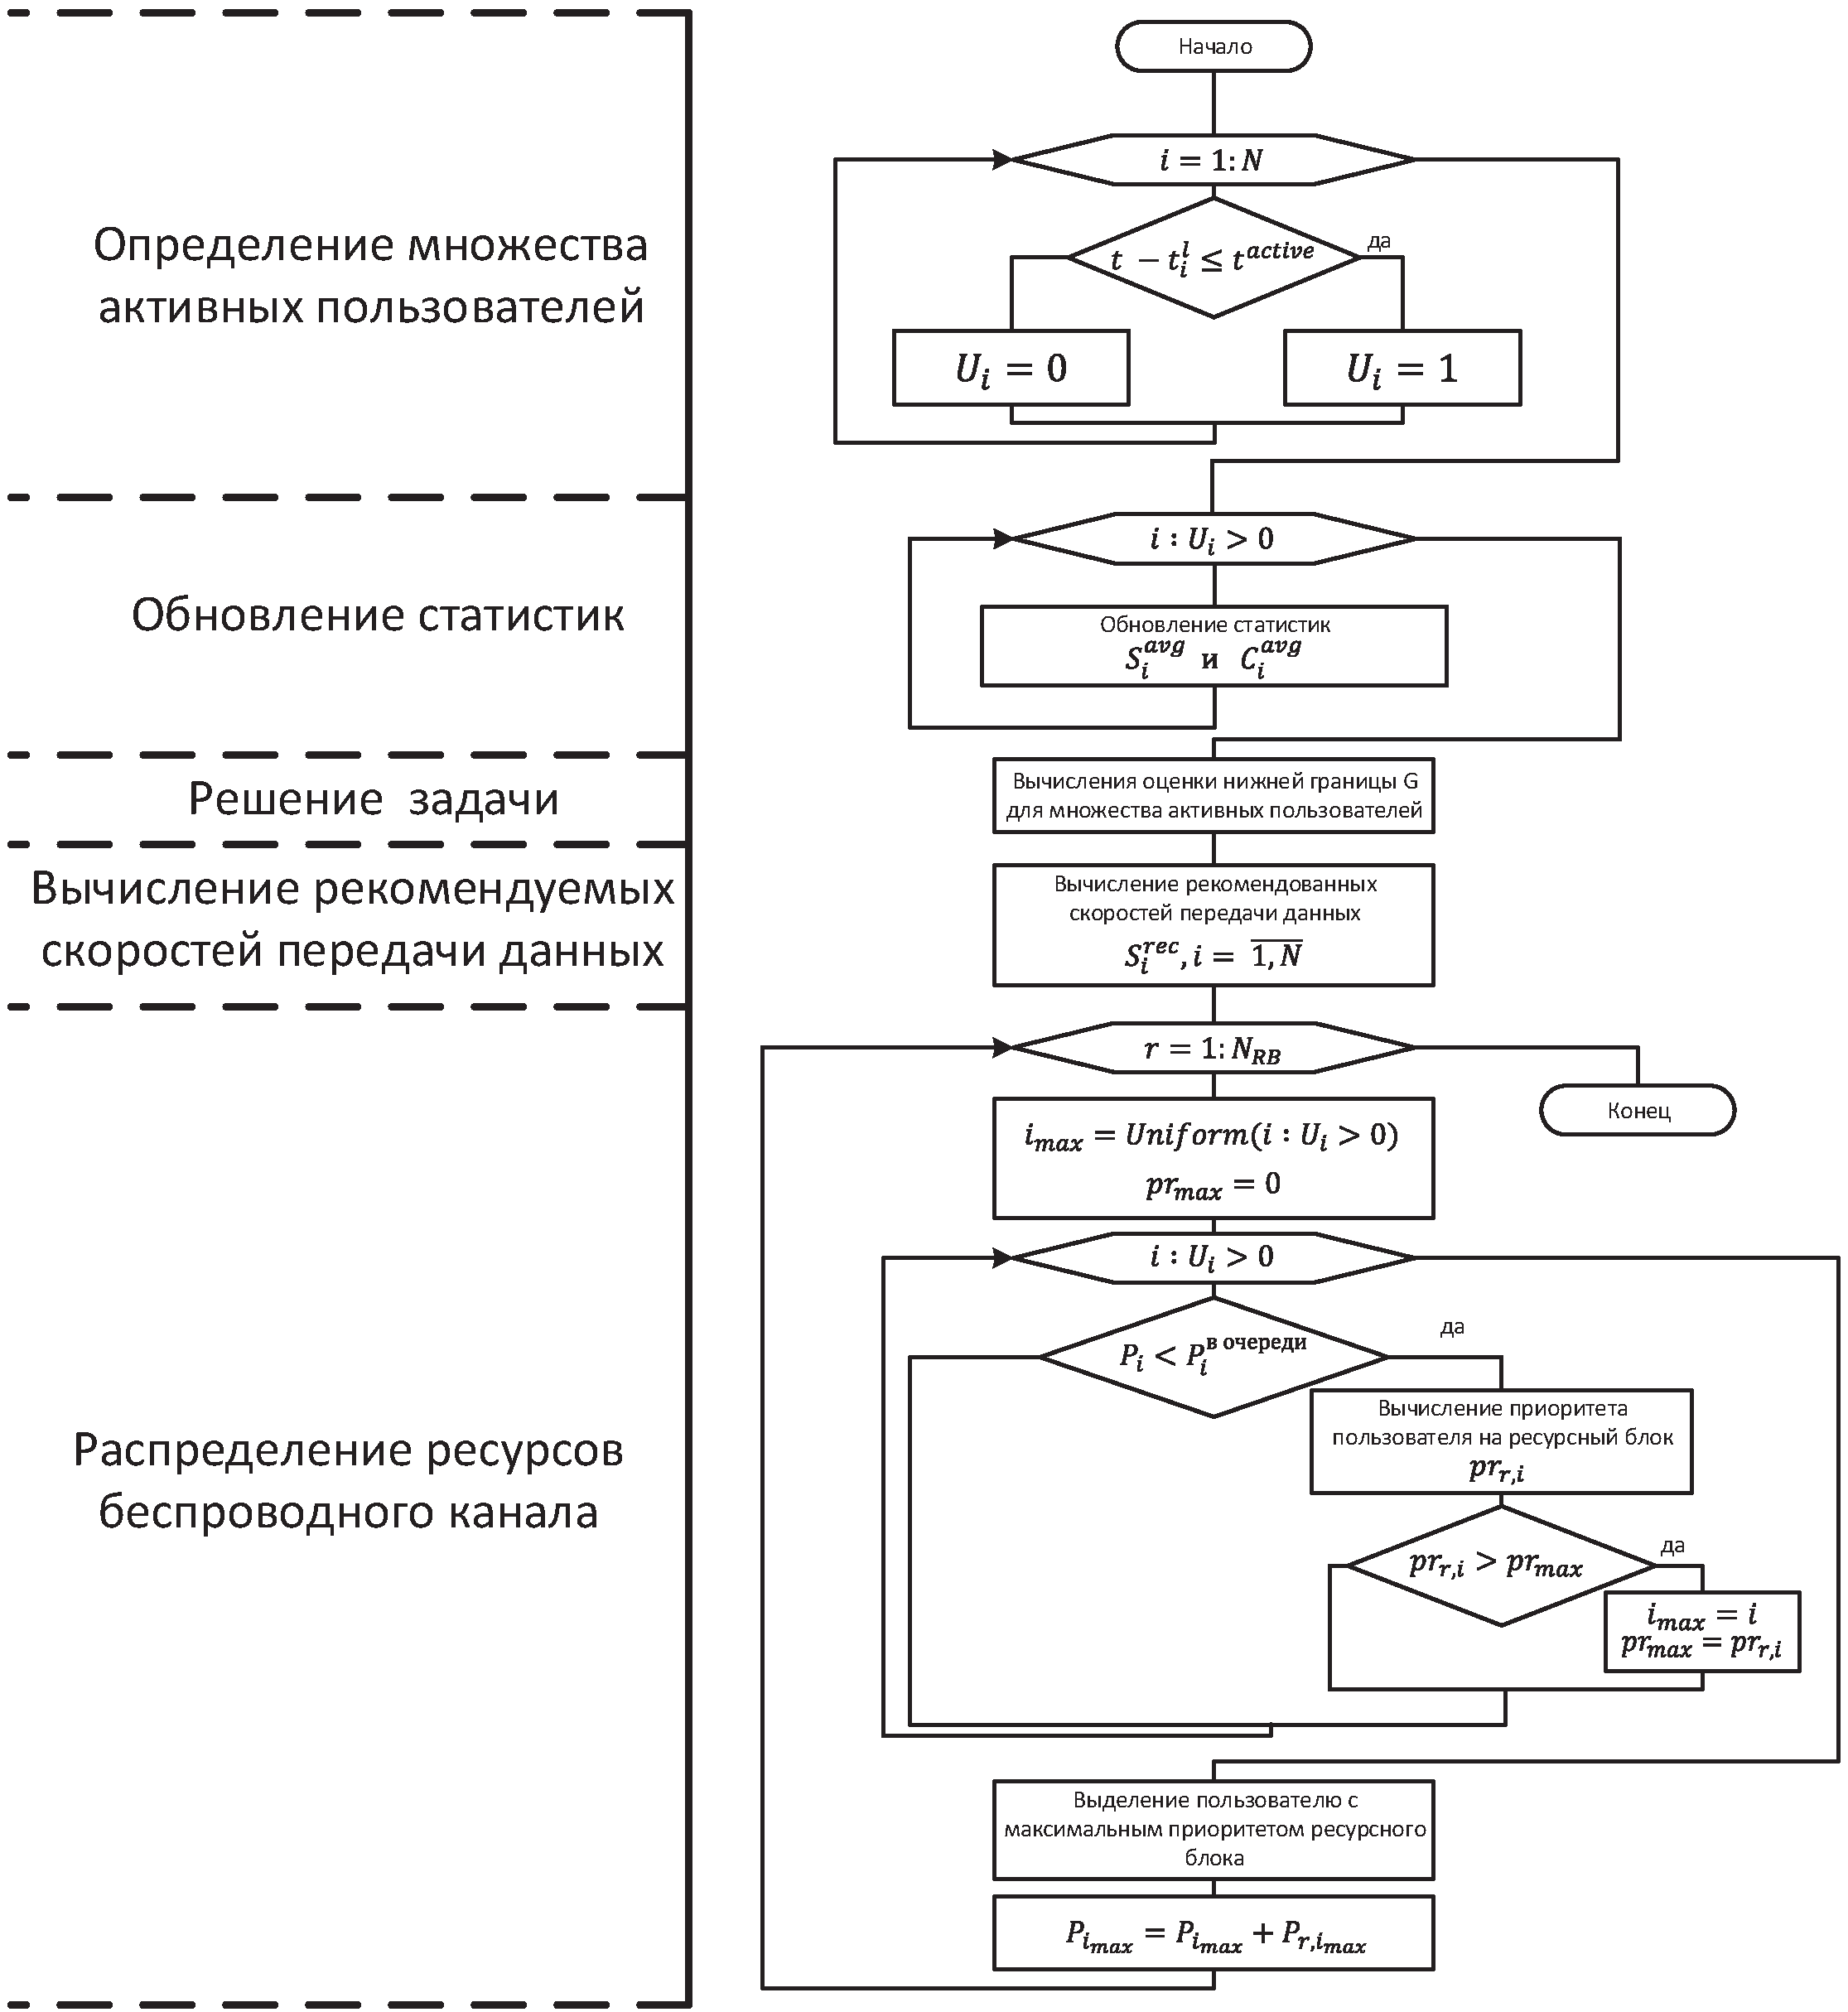
\includegraphics[width=\textwidth]{/Chapter3/hScheduler.pdf}
\caption{Логика алгоритма совместного планирования распределения ресурсов для неадаптивных видеопотоков}
\label{fig:HScheduler}
\end{center}
\end{figure}

Используя представленные результаты, предлагается алгоритм планирования, выполняемый в каждый интервал планирования, и состоящий из пяти шагов (рисунок~\ref{fig:HScheduler}):
\begin{itemize}
	\item \textbf{Определение множества активных пользователей}. На данном шаге все пользователи разделяются на два подмножества: активные и неактивные, в соответствии с выражением (\ref{eq:activityEstimation}).
	\item \textbf{Обновление статистик}. Для множества активных абонентов обновляются значения статистик в соответствии с выражениями (\ref{eq:CEstimation}) и (\ref{eq:SEstimation}).
	\item \textbf{Решение оптимизационной задачи}. Нахождение решения оптимизационной задачи (\ref{eq:optim_problem_g}) для множества активных пользователей пользователей: $\hat{G}(t) = \{\hat{g}_i(t), i \in \mathcal{U}\}$, при $K_i = \hat{R_i}(t) / C^{avg}_i(t)$ и $\gamma = 1$;
	\item \textbf{Вычисление рекомендуемых скоростей передачи данных}. Вычисление рекомендуемых скоростей передачи данных для всех активных пользователей в соответствии с выражением (\ref{eq:SReqCalc}).
	\item \textbf{Распределение ресурсов беспроводного канала}. Выделение ресурсов беспроводного канала в соответствии с предложенным механизмом обеспечения рекомендованной скорости (\ref{eq:PriorFunction}). На данном шаге также производится контроль за объемом выделенных ресурсов с целью предотвращения выделения ресурсных блоков, которые не могут быть использованы пользователем ввиду отстутствия информации в очереди на базовой станции.
\end{itemize}

В результате настоящего подраздела был предложен алгоритм планирования распределения частотно-временных ресурсов беспроводного канала связи для централизованных систем передачи информации. Производительность предложенного алгоритма планирования будет продемонстрирована в подразделе \ref{chap3:NumericalExample}.

\section{Численный пример}
\label{chap3:NumericalExample}

Демонстрация результатов настоящей работы является нетривиальной задачей ввиду сложности анализируемой системы и невозможности постановки натурных экспериментов, так как оборудование централизованных сетей связи (базовые станции, опорная сеть оператора и т.д.) недоступно для рядового исследователя, что приводит к необходимости поиска платформы для моделирования. Таким образом, настоящий подраздел решает две задачи:
\begin{itemize}
	\item Выбор стандарта беспроводной централизованной системы передачи информации, на котором будут демонстрироваться полученные результаты;
	\item Выбор платформы и сценария моделирования.
\end{itemize}

Проведем анализ современных стандартов связи, которые соответствуют рассматриваемой в настоящей работе модели системы (раздел \ref{chap2}). В настоящий момент времени наиболее известными технологиями, котрые соответствуют введенной модели системы, являются два стандарта связи: IEEE 802.16 или \textit{Worldwide Interoperability for Microwave Access} (WiMAX) \cite{wimax_std} и \textit{Long-Term Evolution Advanced} (LTE) \cite{lte_std}. Компанией Cisco был проведен анализ распространенности технологий связи, утверждающий что в настоящее время сети связи, построенные на основе стандарта WiMAX, не имеют широкого распространения, а системы стандарта LTE получили широчайшее распространение в мире \cite{Cisco}. Более того, стандарт связи LTE постоянно обновляется и дополняется. Таким образом, результаты настоящей работы будут демонстрироваться на основе стандарта связи LTE. Важно отметить, что все полученные результаты применимы ко всем беспроводным централизованным системам связи, а в данном разделе лишь демонстрируются на примере самого распространенного стандарта, удовлетворяющего модели системы.

Следующим шагом необходимо выбрать платформу моделирования систем стандарта LTE. В настоящий момент времени существует несколько возможных платформ:
\begin{itemize}
	\item \textit{Maltab}. Компанией MathWorks предлагается модуль анализа сетей стандарта LTE: LTE System Toolbox в рамках пакета Simulink, распространяемый с платной подпиской \cite{Matlab}. Данный модуль позволяет оценивать характеристики беспроводного канала связи путем имитационного моделирования. Однако, в настоящем пакете не представлены реализации вышележащих уровней: стека протоколов беспроводного соединения стандарта LTE и опорной сети оператора. Это приводит к невозможности использования данной платформы для демонстрации результатов настоящей работы.
	\item \textit{Opnet LTE Simulation}. Компания Opnet предлагает платформу для моделирования сетей стандарта LTE с платной подпиской OPNET LTE SIMULATION \cite{Opnet}. Данная платформа включает в себя полный стек проколов беспроводной связи и опорной сети оператора. Однако, исходный код данного проекта является закрытым и его невозможно дополнить клиент-серверными приложениями, осуществляющими загрузку и демонстрацию видео. Следовательно, использовать данну платформу невозможно для демонстрации полученных результатов.
	\item Система моделирования \textit{NS-3}. В 2012 году была создана низкоуровневая система моделирования сетевых протоколов с открытым исходным кодом NS-3 \cite{ns-3}. Данная система моделирования реализована на языке программирования С++, и ее компоненты соответствует стандартам связи. В NS-3 также реализован модуль стека протоколов LTE для беспроводной сети и опорной сети оператора, соответствующий стандарту \cite{lte_std}. Открытый исходный код позволяет производить дополнение и гибкую настройку системы для широкого спектра задач.
\end{itemize}

Таким образом, результаты настоящей работы будут демонстрироваться в системе моделирования NS-3 для стандарта связи LTE. Достоверность полученных результатов обеспечивается соответствием системы моделирования и ее компонентов стандарту связи LTE и DASH.

Для адаптации системы моделирования NS-3 для демонстрации результатов настоящей работы был решен ряд технических задач:
\begin{itemize}
	\item Реализация видео контент сервера и клиентского приложения, соответствующих стандарту DASH (подраздел \ref{chap1:VideoPlayers});
	\item Реализация в модуле базовой станции LTE системы анализа трафика DPI, которая позволяет в каждый момент времени моделирования получить информацию о виде трафика и его характеристиках;
	\item Реализация механизмов оценки характеристик беспроводной сети передачи информации в соответствии с решениями, представленными в подразделе \ref{chap3:NonAdaptiveScheduler};
	\item Реализация алгоритма планирования, предложенного в подразделе \ref{chap3:NonAdaptiveScheduler}.
\end{itemize}

Следующим важным шагом для демонстрации результатов является выбор сценария моделирования. В настоящей работе использовались указания, представленные в \cite{simulation}. Рассматривается работа одной соты, в которой находится $N$ пользователей на прямой линии с равным расстояниям друг от друга (рисунок \ref{fig:scenario}). Расстояние между соседними пользователями вычисляется следующим образом:
$$\Delta x = \frac{X_{max}}{N+1},$$
где $X_{max}$~--~максимально возможная удаленность пользователей от базовой станции.

\begin{figure}[htbp]
\begin{center}
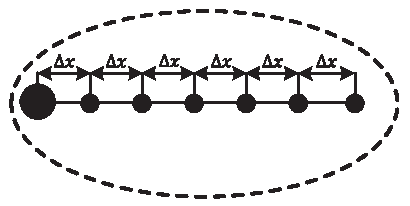
\includegraphics[width=0.7\textwidth]{/Chapter3/scenario.pdf}
\caption{Сценарий моделирования}
\label{fig:scenario}
\end{center}
\end{figure}

В данном сценарии моделирования рассматривается канал связи с плоскими замираниями (подраздел \ref{chap2:RadioChannel}). % Для этого был сгенерирован случайный процесс, который изменяет затухание в канале от времени по всем доступным частотам для передачи. Таким образом затухание сигнала в канале от времени зависит от двух факторов: удаленности от базовой станции и плоскими замираниями в канале связи.
Полный список настроек сценария моделирования для каждого компонента модели системы представлен в таблице \ref{tab:SimParams}.

В сценарии моделирования увеличивалось число абонентов до перехода системы в состоянии перегрузки (определение \ref{def:Congestion}). Далее производилось сравнение производительности известных алгоритмов планирования (\textit{Proportional Fair} и \textit{Round Robin}) с предложенным алгоритмом и найденной нижней границей для критерия $G$ (\ref{eq:gMetricGoal}). Результат проведенного сравнения представлен на рисунке \ref{fig:G_PLOT}.

\begin{figure}[htbp]
\begin{center}
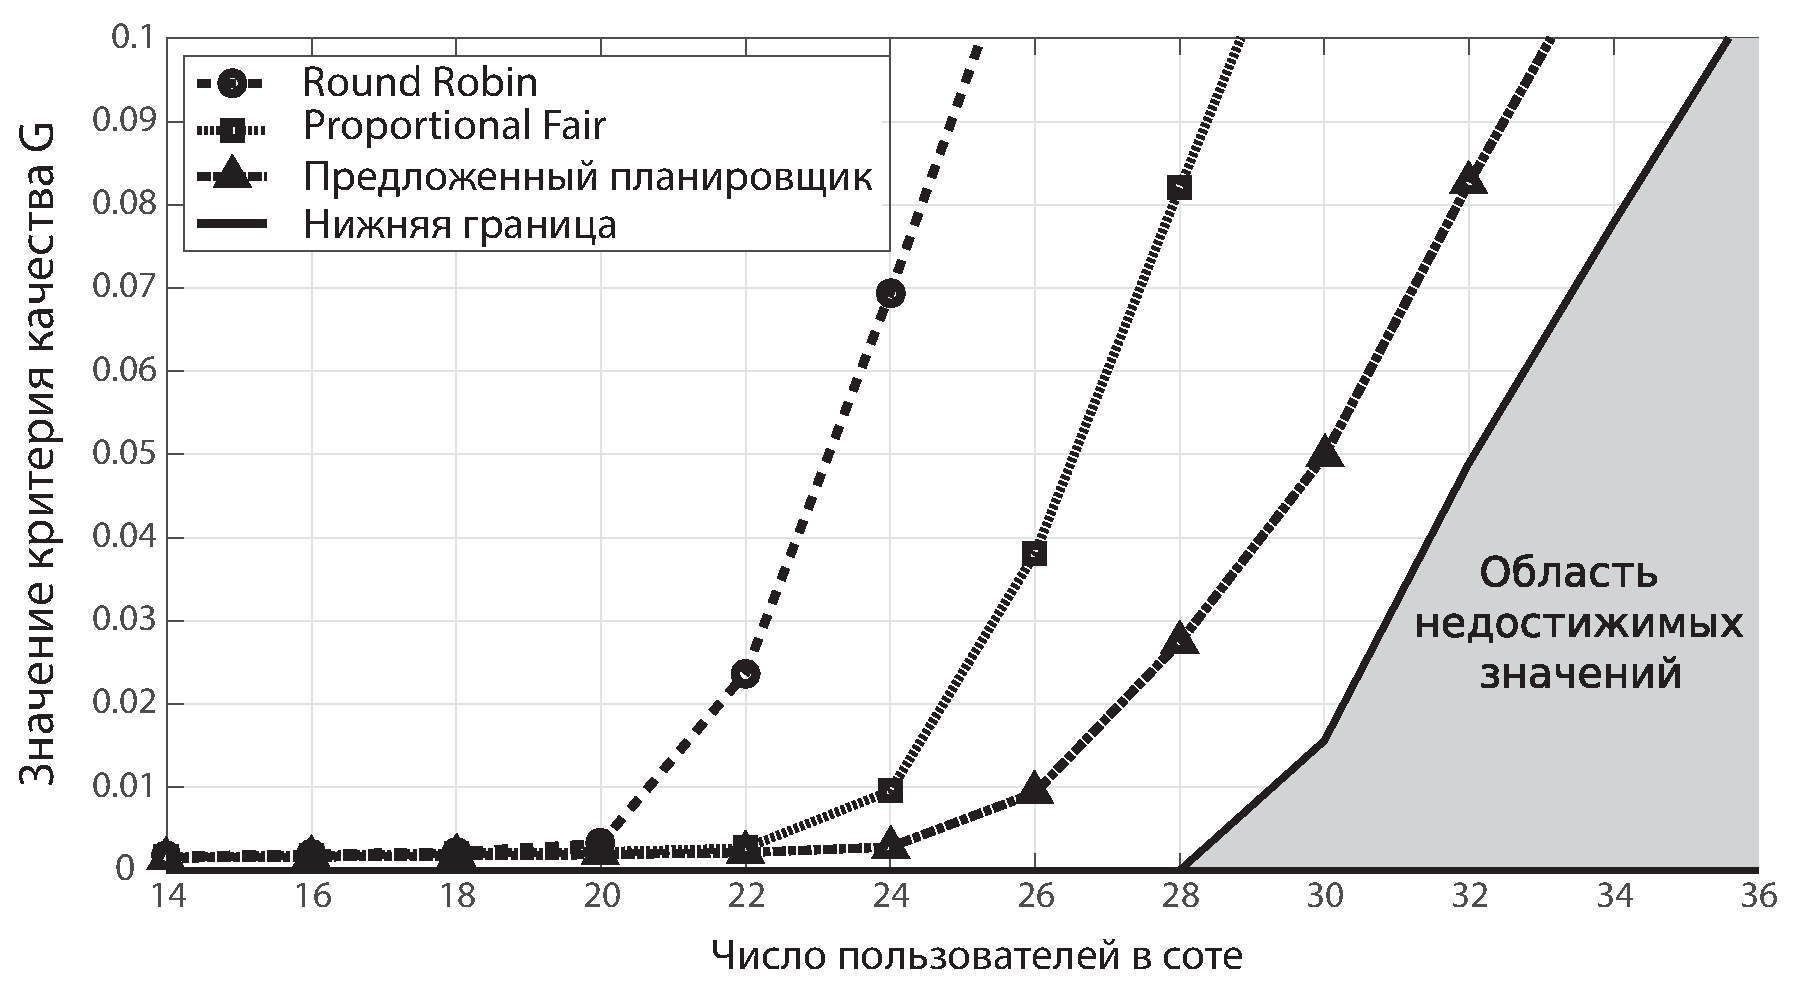
\includegraphics[width=\textwidth]{/Chapter3/G_PLOT.pdf}
\caption{Сравнение предложенного алгоритма планирования с известными планировщиками и найденной нижней границей}
\label{fig:G_PLOT}
\end{center}
\end{figure}

На рисунке \ref{fig:G_PLOT} приведена нижняя граница, характеризующая максимальную производительность алгоритмов планирования в настоящем сценарии моделирования. Заштрихованная область характеризует значения, которые не могут быть достигнуты любым планировщиком, удовлетворяющим допущениям введенных в подразделе \ref{chap2:Assumptions}: не существует планировщика, который при 30-ти пользователей в соте обеспечивает значения критерия качества восприятия $G$ равный $0.01$. Из рассмотрения рисунка \ref{fig:G_PLOT} следует, что предложенный алгоритм планирования показывает производительность на 7-14\% выше по числу удовлетворенных пользователей при заданном уровне качества обслуживания в сравнении со стандартными алгоритмами. Более того производительность предложенного планировщика близка к нижней границей.

\section{Выводы по разделу}

Настоящий раздел был посвящен вопросам анализа и увеличения производительности беспроводных централизованных сетей для передачи неадаптивных видеопоследовательностей. В рамках раздела был выбран критерий качества восприятия для неадаптивного видеопотока: нормированное отношение длительностей буферизации и просмотра (определение \ref{def:gMetric}), и произведен его анализ. На основании данного критерия и модели системы, введенной в разделе \ref{chap2}, была поставлена оптимизационная задача нелинейного программирования (\ref{eq:optim_problem_g}), решение которой характеризует максимально возможную производительность алгоритмов планирования при передаче неадаптивного видео. Далее было предложено решение данной задачи, путем ее сведения к обобщению непрерывной задачи о рюкзаке, решение которого было найдено в настоящем разделе. Полученное решение характеризует нижнюю границу нормированного отношения длительностей буферизации и просмотра для всевозможных алгоритмов планирования, удовлетворяющих введенных допущениям в подразделе \ref{chap2:Assumptions}, при передаче неадаптивных видеопотоков.

На основе найденного решения, обладающего низкой вычислительной сложностью, был предложен планировщик, обладающий высокой производительностью в сравнении с существующими планировщиками и найденной нижней границей.

Основные результаты раздела могут быть сформулированы следующим образом:
\begin{itemize}
	\item Проведен анализ факторов, влияющих на восприятие неадаптивных видепотоков. Выбран критерий качества восприятия неадаптивных видеопотоков на основе нормированного отношения длительностей буферизации и просмотра (подраздел~\ref{chap3:NonAdaptiveQoe});
	\item Произведена постановка оптимизационной задачи нелинейного программирования, характеризующей нижнюю границу для введенного критерия. Найдено ее решение и предложен алгоритм расчета нижней границы для нормированного отношения длительностей буферизации и просмотра по всевозможным алгоритмам планирования, удовлетворяющим допущениям из подраздела \ref{chap2:Assumptions} (подразделы \ref{chap3:NonAdaptiveOptimizationProblem}, \ref{chap3:GeneralizedFKSP} и \ref{chap3:LowerBoundForG});
	\item Предложен алгоритм планирования для неадаптивных видеопотоков, реализующий концепцию совместного планирования распределения ресурсов на базовой станции. Показано, что производительность предложенного планировщика превосходит известные решения на 7-14\% и сравнима с нижней границей. Результаты настоящего раздела демонстрировались в системе моделирования NS-3 для стандарта связи LTE, соответствующего модели системы передачи информации, введенной в разделе \ref{chap2} (подразделы \ref{chap3:NonAdaptiveScheduler} и \ref{chap3:NumericalExample}).
\end{itemize}
